\documentclass[12pt]{report}
\usepackage[fontsize=13pt]{scrextend}
\usepackage[utf8]{vietnam}
\usepackage[utf8]{inputenc}
\usepackage[vietnamese]{babel}
\usepackage{titlesec}
\usepackage{titletoc}
\usepackage{listings}
\usepackage[bookmarks=true]{hyperref}
\usepackage[left=3cm,right=2cm,top=2.5cm,bottom=3cm]{geometry}
\usepackage{graphicx}
\usepackage{hyperref}
\usepackage{tabularx}
\usepackage{tikz}
\usepackage{varwidth}
\usepackage{float}
\usepackage{longtable}
\usepackage{listings}
\usepackage{color}
\usepackage{multirow}
\usepackage{booktabs}
\usepackage[ruled,vlined]{algorithm2e}
\usepackage{chngcntr}
\usepackage{nameref}

%\usepackage[font=bf]{caption}
%\counterwithin{figure}{chapter}

\renewcommand\labelitemi{--}

\setlength{\parskip}{6pt}

\usetikzlibrary{calc}
\setlength{\parindent}{10mm}
\renewcommand{\baselinestretch}{1.3}
\graphicspath{{images/}}

%%% The following lines add Chapter or Appendix in front of the number
\titlecontents{chapter}%
[0pt]%
{\vspace{1ex}}%
{\bfseries Chương \thecontentslabel\quad}%
{\bfseries}%
{\bfseries\hfill\contentspage}
%%% Initially, for the main part of the document, set the label to "Chapter"
\let\chapappname\chaptername

\definecolor{dkgreen}{rgb}{0,0.6,0}
\definecolor{gray}{rgb}{0.5,0.5,0.5}
\definecolor{mauve}{rgb}{0.58,0,0.82}

% setup code area as listings
\lstset{frame=tb,
  language=Java,
  aboveskip=3mm,
  belowskip=3mm,
  showstringspaces=false,
  columns=flexible,
  basicstyle={\small\ttfamily},
  numbers=left,
  numberstyle=\tiny\color{gray},
  keywordstyle=\color{blue},
  commentstyle=\color{dkgreen},
  stringstyle=\color{mauve},
  breaklines=true,
  breakatwhitespace=true,
  tabsize=3
}

\renewcommand{\lstlistingname}{Mã nguồn}

\newenvironment{thuattoan}[1][h]
  {\renewcommand{\algorithmcfname}{Thuật toán}
   \begin{algorithm}[#1]
  }{\end{algorithm}}

% hyper setup
\hypersetup{
	bookmarks=true,
	pdftitle={Xây dựng hệ thống back-end trong phần mềm đa nền tảng IQ-TREE giao diện đồ họa người dùng},
	pdfauthor={Nguyễn Đăng Nam}, % author
	pdfsubject={TeX and LaTeX},
	pdfkeywords={TeX, LaTeX, graphics, images}, % list of keywords
	colorlinks=false,       % false: boxed links; true: colored links
	linkcolor=black,       % color of internal links
	citecolor=black,       % color of links to bibliography
	filecolor=black,        % color of file links
	urlcolor=black,        % color of external links
	linktoc=page            % only page is linked
}

\begin{document}
\begin{titlepage}
	\center
	\begin{tikzpicture}[overlay,remember picture]
		\draw [line width=3pt,rounded corners=0pt,]
		($ (current page.north west) + (25mm,-25mm) $)
		rectangle
		($ (current page.south east) + (-15mm,25mm) $);
		\draw [line width=1pt,rounded corners=0pt]
		($ (current page.north west) + (26.5mm,-26.5mm) $)
		rectangle
		($ (current page.south east) + (-16.5mm,26.5mm) $);
	\end{tikzpicture}
	
	{\large \bfseries ĐẠI HỌC QUỐC GIA HÀ NỘI\\ TRƯỜNG ĐẠI HỌC CÔNG NGHỆ}\\[1cm]
	
\includegraphics[width=0.2\linewidth]{Image/UET.png}\\[1cm]
	{\Large  \bfseries Nguyễn Đăng Nam}\\[1.5cm]
	{ \LARGE \bfseries XÂY DỰNG HỆ THỐNG BACK-END TRONG PHẦN MỀM ĐA NỀN TẢNG IQ-TREE \\ GIAO DIỆN ĐỒ HỌA NGƯỜI DÙNG}\\[0.5cm]
	\hfill\\[1.5cm]
	{\large \bfseries KHÓA LUẬN TỐT NGHIỆP ĐẠI HỌC HỆ CHÍNH QUY}\\	
	{\large \bfseries Ngành: Công nghệ thông tin}	
	\hfill\\[1.5cm]	
	{\large \bfseries HÀ NỘI - 2022}\\	
	\vfill
\end{titlepage}
	
%-----SECONDARY TITLE PAGE-----%	
\begin{titlepage}
	\center
	\begin{tikzpicture}[overlay,remember picture]
		\draw [line width=3pt,rounded corners=0pt,]
		($ (current page.north west) + (25mm,-25mm) $)
		rectangle
		($ (current page.south east) + (-15mm,25mm) $);
		\draw [line width=1pt,rounded corners=0pt]
		($ (current page.north west) + (26.5mm,-26.5mm) $)
		rectangle
		($ (current page.south east) + (-16.5mm,26.5mm) $);
	\end{tikzpicture}
	
	{\large \bfseries ĐẠI HỌC QUỐC GIA HÀ NỘI\\ TRƯỜNG ĐẠI HỌC CÔNG NGHỆ}\\[2cm]

	{\Large  \bfseries Nguyễn Đăng Nam}\\[2cm]		
	{ \LARGE \bfseries XÂY DỰNG HỆ THỐNG BACK-END TRONG PHẦN MỀM ĐA NỀN TẢNG IQ-TREE \\ GIAO DIỆN ĐỒ HỌA NGƯỜI DÙNG}\\[0.5cm]
	\hfill\\[1.5cm]
	{\large \bfseries KHÓA LUẬN TỐT NGHIỆP ĐẠI HỌC HỆ CHÍNH QUY}\\	
	{\large \bfseries Ngành: Công nghệ thông tin}
	\hfill\\[2cm]
	\begin{flushleft}
		{\large \bfseries Cán bộ hướng dẫn: TS. Hoàng Thị Điệp}\\	
	\end{flushleft}
	\hfill\\[2cm]		
	{\large \bfseries HÀ NỘI - 2022}\\		
	\vfill		
\end{titlepage}

%-----THANKS-----%
\newpage
\pagenumbering{roman}
\begin{center}
	\textbf{\large LỜI CẢM ƠN}
\end{center}

Lời đầu tiên, em xin dành lời cảm ơn chân thành đến  TS.Hoàng Thị Điệp. Trong quá trình làm khóa luận em đã nhận được sự hướng dẫn nhiệt tình và chu đáo từ cô. Những lời khuyên và kiến thức được truyền đạt đóng góp rất lớn trong khóa luận của em. Chưa dừng ở đó, cô cũng rất hỗ trợ em trong quá trình định hướng cũng như chỉ ra những vấn đề thiếu sót của bản thân em để cho em ngày một hoàn thiện bản thân mình một cách tốt hơn.

Để có thể phát triển sản phẩm thật tốt, em xin được gửi lời cảm ơn đến các thành viên cùng phát triển các mô-đun của sản phẩm là bạn Nguyễn Thành Đạt, bạn Hoàng Văn Giáp, em Võ Minh Đức. Nhờ sự góp sức và đóng góp của mọi người, mình không cảm thấy cô đơn và có những người đồng hành thật tốt bụng cũng như tính cống hiến, đóng góp cao. 

Em xin cảm ơn Ban lãnh đạo và các giảng viên của Trường Đại học Công Nghệ - Đại học Quốc Gia Hà Nội đã tạo điều kiện cho em được học tập tại một môi trường chất lượng và truyền đạt những kinh nghiệm và kiến thức quý báu cho em. Bên cạnh đó, tôi xin gửi lời cảm ơn đến bạn bè - những người đã luôn động viên tôi. Trong đó không thể không kể đến tập thể K63-CB đã luôn bên cạnh giúp đỡ tôi trong suốt quá trình làm khóa luận. Các bạn đã đem đến cho tôi những kỷ niệm thật là khó quên. Bốn năm được học cùng các bạn là khoảng thời gian vui vẻ của tôi.

Em xin chân thành cảm ơn thầy/cô phản biện đã dành thời gian ra đọc và phản biện khóa luận của em, giúp cho em có thêm những bài học và tiến bộ hơn. Em xin cảm ơn sâu sắc đến quý thầy/cô.
Mặc dù đã cố gắng hết sức , tuy nhiên khóa luận chắc chắn vẫn còn những hạn chế, thiếu sót, kính mong nhận được chỉ bảo, góp ý của các thầy cô để em tiếp tục hoàn thiện nội dung nghiên cứu và hoàn thiện khóa luận.

Một lần nữa, xin chân thành cảm ơn tất cả mọi người.


	
%-----ABSTRACT-----%
\newpage
\begin{center}
	\textbf{\large TÓM TẮT}
\end{center}

Hiện nay, với sự bùng nổ của công nghệ thông tin cũng như số lượng máy tính ngày càng tăng vọt, nhu cầu sử dụng máy tính cho công việc của mọi người đều tăng lên. Với mỗi phần mềm,người dùng luôn có kỳ vọng về một phần mềm giao diện, dễ thao tác, dễ sử dụng và mang lại một trải nghiệm tốt cũng như tiết kiệm thời gian. Những phần mềm hướng đến cộng đồng nghiên cứu cơ bản nói chung và sinh học, sinh học tiến hóa nói riêng cũng không phải ngoại lệ. Hiện nay, IQTREE là một trong số những phần mềm phổ biến về suy luận cây tiến hóa theo tiêu chuẩn hợp lý cực đại (ML) và được cộng đồng nghiên cứu sinh học quan tâm. Tuy nhiên, phần mềm IQTREE là phần mềm dòng lệnh nên gây ra khó khăn cho những người mới tiếp cận, nhất là đối với các nhà nghiên cứu sinh học (những người ít có nền tảng về dòng lệnh máy tính). Vậy nên chúng tôi đề xuất phát triển phần mềm GIQ-TREE là phần mềm giao diện đồ họa người dùng đa nền tảng có thể chạy trên các hệ điều hành phổ biến hiện nay như Windows, Linux, MacOS.\\

\noindent \textit{\textbf{Từ khóa:} IQTREE, giao diện đồ họa người dùng, cây tiến hóa, suy luận tiến hóa}

%-----UNDERTAKING-----%
\newpage
\begin{center}
	\textbf{\large LỜI CAM ĐOAN}
\end{center}

Tôi xin cam đoan khóa luận tốt nghiệp “Xây dựng hệ thống back-end trong phần mềm đa nền tảng IQ-TREE giao diện đồ họa người dùng” là công trình nghiên cứu của riêng tôi và được sự hướng dẫn của TS. Hoàng Thị Điệp và chưa từng được nộp như một báo cáo khóa luận tại trường Đại học Công nghệ - Đại học Quốc Gia Hà Nội hoặc bất kỳ trường đại học khác. Những gì tôi viết ra không sao chép từ các tài liệu, không sử dụng các kết quả của người khác mà không trích dẫn cụ thể.

Tôi xin cam đoan những nội dung tôi trình bày trong khóa luận là do tôi tự phát triển, không sao chép mã nguồn của người khác. Nếu sai tôi hoàn toàn chịu trách nhiệm theo quy định của trường Đại học Công nghệ - Đại học Quốc Gia Hà Nội.
.\\

\begin{flushright}
	\begin{varwidth}{\linewidth}\centering
		Hà Nội, ngày 30 tháng 04 năm 2022\\
		Sinh viên\\[2cm]
		Nguyễn Đăng Nam
	\end{varwidth}
\end{flushright}

%-----TOC-----%
\newpage
\tableofcontents

\newpage
\addcontentsline{toc}{chapter}{\listtablename}
\listoftables

\newpage
\addcontentsline{toc}{chapter}{Danh sách ký hiệu, chữ viết tắt}
\begin{flushleft}
\bfseries{\Huge{Danh sách ký hiệu, chữ viết tắt}}
\end{flushleft}
\begin{table}[h]
	\centering
	\begin{tabular}{lll}
	    \textbf{Từ viết tắt}  & Từ đầy đủ & Ý nghĩa \\[0.3cm]
		\textbf{DNA}  & Deoxyribonucleic acid & Phần tử mang thông tin di truyền \\[0.3cm]
		\textbf{ML}  & Maximum Likelihood  & Tiêu chuẩn hợp lý cực đại \\[0.3cm]
		\textbf{MP}  & Maximum Parsimony & Tiêu chuẩn tiết kiệm nhất \\[0.3cm]
		\textbf{RAM}  & Random access memory & Bộ nhớ mềm \\[0.3cm]
		\textbf{SEO}  & Search engine optimization  & kiếm \\[0.3cm]
		\textbf{CMS}  & Content management system & Hệ thống quản trị nội dung \\[0.3cm]
		\textbf{SPA}  & Single Page Application & Ứng dụng đơn trang \\[0.3cm]
		\textbf{JSON}  & JavaScript Object Notation & Kiểu dữ liệu theo từ khóa-giá trị \\[0.3cm]
		\textbf{UI}  & User Interface  & Giao diện người dùng \\[0.3cm]
		\textbf{UX}  & User Experience  & Trải nghiệm người dùng \\[0.3cm]
		\textbf{GUI}  & Graphical User Interface & Giao diện đồ họa người dùng \\[0.3cm]
		\textbf{CPU}  & Central processing unit & Bộ xử lý trung tâm \\[0.3cm]
		\textbf{OTUs}  & Operational taxonomic units & Đơn vị phân loại hoạt động \\[0.3cm]
		\textbf{HTUs}  & Hypothetical taxonomic units & Đơn vị phân loại giả thuyết  \\[0.3cm]
	\end{tabular}
\end{table}

\newpage
\addcontentsline{toc}{chapter}{\listfigurename}
\listoffigures

%-----MAIN-----%
\newpage
\pagenumbering{arabic}
\setcounter{page}{1}
\chapter{Mở đầu}
\label{chap:intro}
\section{Tính cấp thiết}
Trong thế kỷ XXI, máy tính đang dần trở lên ngày càng phổ biến và việc sử dụng máy tính ngày càng trở nên đại trà hơn trên toàn thế giới. Người dùng mới luôn gặp khó khăn trong việc tiếp cận với các dòng lệnh máy tính để thực hiện những thao tác mà họ muốn sử dụng trên máy tính cá nhân. Để hỗ trợ người dùng phổ thông, các phần mềm giao diện đồ họa người dùng là việc tất yếu cần phát triển để tối ưu hóa thời gian làm quen, sử dụng và mang lại trải nghiệm tốt cho người dùng. Các phần mềm giao diện đồ họa người dùng sẽ trợ giúp con người những bước “khô khan” như học thuộc và thao tác các câu lệnh. Với lập trình viên, chúng ta có những ngôn ngữ bậc cao giúp việc lập trình dễ hơn. Còn với người dùng, chúng ta có phiên bản giao diện đồ họa người dùng, giúp người dùng sử dụng dễ hơn.
Bên cạnh việc tin học là việc thứ yếu đang dần trở thành thiết yếu, từ xưa đến nay, sinh học vẫn luôn là những thứ thiết yếu liên quan đến sự tồn tại của loài người nói riêng và quần thể sinh học nói chung. Trong thế kỷ XXI, rất nhiều lần chúng ta phải đối mặt với các đại dịch nguy hiểm mang tính toàn cầu, gần đây nhất là đại dịch COVID-19 do virus SARS-CoV-2 gây ra. Điều này như một luận cứ củng cố cho luận điểm bên trên. Các nhà nghiên cứu đã nghiên cứu và phát triển từ lâu một lĩnh vực nghiên cứu mang tên Tin sinh học nhằm tận dụng sức mạnh tính toán của máy tính để hỗ trợ cho nghiên cứu sinh học. Sinh học tiến hóa là một nhánh nổi bật trong đó.

IQTREE là một phiên bản dòng lệnh hỗ trợ thực hiện các phân tích và suy luận tiến hóa áp dụng rất nhiều công trình và thuật toán tốt trên thế giới. Với sự phát triển và phổ biến của phần mềm IQTREE, việc sử dụng dòng lệnh là khó khăn cho những người dùng phổ thông mới tiếp cận hay cho những nhà nghiên cứu sinh học. Vậy nên, phiên bản giao diện đồ họa người dùng là cần thiết với IQTREE để mang lại trải nghiệm tốt cho người dùng nói chung cũng như tiết kiệm thời gian cho cộng đồng nghiên cứu sinh học nói riêng. 
\section{Nội dung tiến hành}
Mục tiêu chính của khóa luận này là xây dựng hệ thống bạck-end của ứng dụng GIQ-TREE - phiên bản giao diện đồ họa người dùng của IQTREE. GIQ-TREE hướng đến việc hỗ trợ đưa IQTREE đến với đông đảo người dùng hơn cũng như là một công cụ hỗ trợ phần nào cho những nghiên cứu của các nhà nghiên cứu sinh học.
\section{Giới thiệu bố cục khóa luận}
Phần còn lại của khóa luận sẽ trình bày về tổng quan, cơ bản về suy luận cây tiến hóa, phân tích các yêu cầu và công nghệ sử dụng, xây dựng back-end cho hệ thống GUI, hệ thống thực nghiệm, thảo luận và kết luận. Cụ thể hơn, \textbf{Chương \ref{chap:chapter1}} sẽ trình bày tổng quan bằng cách giới thiệu cây tiến hóa và ứng dụng, các hệ thống phần mềm xây dựng cây tiến hóa hiện nay, phát biểu bài toán và đưa ra tổng quan giải pháp sơ đồ triển khai. \textbf{Chương \ref{chap:chapter2}} sẽ cung cấp các kiến thức lý thuyết cơ bản về suy luận cây tiến hóa thông qua các cách tiếp cận chính xây dựng cây tiến hoá, suy luận cây tiến hóa theo tiêu chuẩn Maximum Likelihood, các mô hình dữ liệu cho đơn gen và đa gen, các kiểm định thống kê đánh giá cây tiến hóa, suy luận thời gian trên cây tiến hóa, và giới thiệu về hệ thống các phần mềm trong IQTREE.
Chương tiếp theo, \textbf{chương \ref{chap:chapter3}} sẽ đưa ra góc nhìn về việc phân tích các yêu cầu chức năng, phi chức năng, các cơ chế phát triển web, từ đó đưa ra giải pháp cho việc phân vùng phát triển front-end và back-end cho ứng dụng GIQ-TREE và các công nghệ áp dụng trong khóa luận.	\textbf{Chương \ref{chap:chapter4}} sẽ đi chi tiết về việc xây dựng back-end cho hệ thống GUI. \textbf{Chương \ref{chap:chapter5}} sẽ đi qua hệ thống thực nghiệm. Cuối cùng là \textbf{chương \ref{chap:chapter6}} mang đến những kết luận của cá nhân em trong quá trình phát triển, cũng như thảo luận về tương lai của GIQ-TREE
\newpage	
\chapter{Tổng quan}
\label{chap:chapter1}
\section{Giới thiệu cây tiến hóa và ứng dụng}
Cây tiến hóa là sơ đồ dạng cây để biểu diễn quan hệ về tiến hóa giữa một số loài để xem những loài nào có quan hệ họ hàng gần hơn \cite{cia-0} \cite{cia-1}  dựa trên những điểm giống và khác nhau trong thông tin di truyền.

Mối quan hệ tiến hóa giữa các loài thường được biểu diễn dưới dạng cây nhị phân với cấu trúc: mỗi lá của cây biểu diễn một loài (cho bởi dữ liệu đầu vào), mỗi đỉnh trong của cây biểu diễn một loài tổ tiên (thường không biết chính xác); mỗi cạnh của cây nối hai đỉnh của cây với nhau và biểu hiện mối quan hệ trực tiếp giữa hai loài ở hai đỉnh đó của cây, độ dài của mỗi cạnh trên cây cho biết khoảng cách tiến hóa giữa chúng (có thể là thời gian hay số lượng biến đổi nucleotide/axit amin). Cây tiến hóa được minh họa như sau:

\begin{figure}[h]
	\centering
	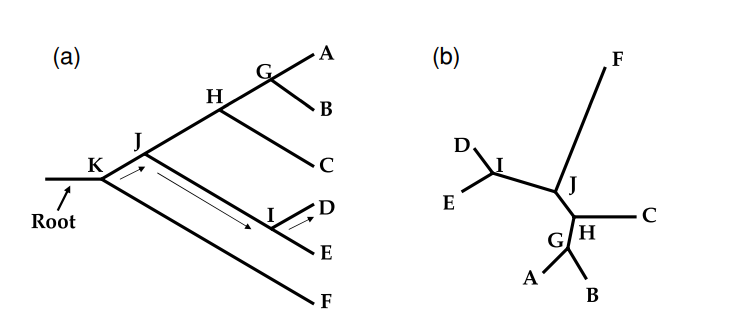
\includegraphics[scale=1]{Image/1.1.png}
	\caption{Hình ảnh minh họa cây tiến hóa \cite{cia-2}}
	\label{fig:image1.1}
\end{figure}

Cây tiến hóa \cite{cia-2} được gọi là cây một phần vì có cấu trúc như một cây gồm các thành phần như gốc, các nhánh, các nốt và các nốt lá. Các nốt bên ngoài (external nodes) hay còn được gọi với cái tên khác là các nốt lá thể hiện đơn vị phân loại và thường được gọi là các OTUs (như các nốt A, B, C, D, E, F). Các nốt trong có thể gọi là HTUs (như các nốt G, H, I, J, K) để thể hiện chúng gần nốt gốc (cha chung) hơn các OTUs. Một nhóm các loài có cùng một nhánh nguyên thủy và có cùng cha chung được gọi là một cụm (cluster). Như \textbf{Hình \ref{fig:image1.1}a }, các loài A, B, C được gọi là cụm khi có chung cha là loài H cũng như có cùng một cây nguyên thủy. 

 Tuy nhiên, trong quá trình tiến hoá, rất khó xác định được tổ tiên chung của các OTUs mà không có thông tin di truyền. Chính vì vậy, rất khó để xác định gốc tổ tiên chung của các loài trên cây. Thay vì thể hiện cây tiến hóa như \textbf{Hình \ref{fig:image1.1}} thì chúng ta nên biểu diễn cây tiến hóa như \textbf{Hình \ref{fig:image1.2}}

\begin{figure}[h]
	\centering
	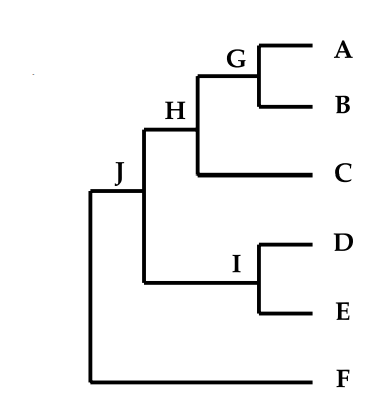
\includegraphics[scale=1]{Image/1.2.png}
	\caption{Hình ảnh minh họa cây nhị phân không gốc \cite{cia-2}}
	\label{fig:image1.2}
\end{figure}

Trong tin sinh học, để dựng được cây tiến hóa, cách làm phổ biến nhất là dựa vào chuỗi DNA/protein của các loài. Lấy ví dụ về nghiên cứu cây tiến hóa trong việc trích rút nguồn gốc của virus, khi virus mới được phát hiện, ta sẽ thực hiện phân tích và thu được cây tiến hóa, từ đó xem virus đó thuộc chủng loài nào và phần nào ước tính được mức độ nguy hiểm mà nó gây ra. Nghiên cứu tìm hiểu sự lây lan của virus đều dựa trên đặc tính sinh học đặc biệt của virus, đó là khi xâm nhập vào vật chủ thì virus vẫn tiếp tục tiến hóa. Vì vậy, cây tiến hóa đóng vai trò then chốt trong những nghiên cứu về virus nói riêng và sinh học tiến hóa nói chung. 

\section{Các hệ thống phần mềm suy luận cây tiến hóa }
Hiện nay trên thế giới có rất nhiều phần mềm và thuật toán xây dựng cây tiến hóa. Dưới đây là bảng thể hiện những ứng dụng xây dựng cây tiến hóa phổ biến (có lượng trích dẫn lớn, đông đảo cộng đồng quan tâm)

\begin{table}[h]
	\centering
	\caption{Bảng các ứng dụng thực hiện phân tích xây dựng cây tiến hóa phổ biến hiện nay}
	\label{tbl:table1.1}
	\begin{tabular}{|p{3cm}|l|l|l|}
		\hline
		\textbf{Phiên bản command-line} & \textbf{Phiên bản web} & \textbf{Phiên bản desktop} \\ \hline
		IQTREE \cite{cia-3}              & W-IQTREE \cite{cia-4}        &                                  \\ \hline
		RAxML \cite{cia-5}             & raxmlGUI \cite{cia-6}      &             raxmlGUI 2.0 \cite{cia-7}                    \\ \hline
		PhyML \cite{cia-8}             & PhyML Online \cite{cia-9}    &                                  \\ \hline
	\end{tabular}
\end{table}

\section{Phát biểu bài toán}
Nhiệm vụ chính của hệ thống back-end là thiết kế giải pháp nhằm hỗ trợ người dùng sử dụng phần mềm một cách hiệu quả mà không cần nhớ những câu lệnh máy tính khô khan hay những tài liệu dày đặc chữ để mô tả cách làm. Từ nhu cầu của người dùng, GIQ-TREE có những đặc điểm riêng biệt:

- Tổ chức thư mục cho mỗi dự án theo cách khoa học, không bị rối như phiên bản tiền nhiệm.

- Cài đặt được thiết kế dưới dạng cây phân cấp nhằm phân chia rõ ràng các vùng cài đặt, qua đó góp phần tăng hiệu suất và trải nghiệm người dùng.

- Hiệu suất phân tích gần như hệt phiên bản IQTREE do đã nhúng phần mềm IQTREE vào bên trong GIQ-TREE

- Các tính năng phổ biến được cài đặt và thiết kế được tham khảo và dựa trên tài liệu của nhóm phát triển IQ-TREE: \url{http://www.iqtree.org/}

\section{Sơ đồ của giải pháp triển khai}
Mục tiêu của việc phát triển logic backend cho GIQ-TREE là một phiên bản ứng dụng được cài đặt trên máy của người dùng, sử dụng những tài nguyên của máy tính họ. Giải pháp của em là ánh xạ các cài đặt của GIQ-TREE sang câu lệnh dòng lệnh của IQTREE, ứng dụng IQTREE như một mô-đun được tích hợp bên trong GIQ-TREE. Khi thực hiện phân tích, thực hiện chuyển đổi ánh xạ các lựa chọn trên giao diện đồ họa sang đối số dòng lệnh để thực hiện. Khi hoàn thành phân tích, chương trình lấy kết quả đầu ra của bản dòng lệnh để đưa cho bên giao diện hiển thị.

Hình ảnh sau đây mô tả trực quan cho giải pháp cho toàn thể ứng dụng chứ không chỉ back-end:

\begin{figure}[h]
	\centering
	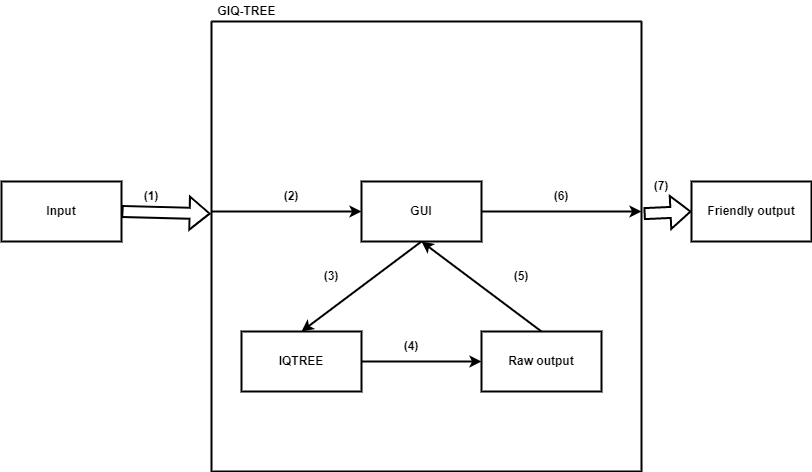
\includegraphics[scale=0.55]{Image/1.3.png}
	\caption{Mô tả trực quan giải pháp}
	\label{fig:image1.3}
\end{figure}

Với giải pháp này, GIQ-TREE có thể đảm bảo hiệu năng phân tích như trên phiên bản tiền nhiệm IQTREE.

\newpage	
\chapter{Cơ bản về suy luận cây tiến hóa}
\label{chap:chapter2}
\section{Suy luận cây tiến hóa và các tiếp cận chính }
Việc tái tạo lại cây tiến hóa từ các chuỗi nucleotide hay amino acid không dễ dàng như kỳ vọng, và việc xác định một cây là hoàn toàn đúng gần như bất khả thi. Mặc dù vậy, có rất nhiều phương pháp đã ra đời để thực hiện suy luận tiến hóa dựa trên xác suất đúng cao và gần giống với cây thật.

Suy luận tiến hóa \cite{cia-10} là việc phân tích và tái dựng lịch sử tiến hóa của các loài liên quan bằng cách nhóm những loài có cùng đặc điểm vào với nhau (với hàm ý chúng có tổ tiên chung). Mục đích của suy luận tiến hóa là để xây dựng một cây tiến hóa về loài để phục vụ cho việc nghiên cứu sinh học. Đầu vào của bài toán là một ma trận biểu diễn sắp hàng các chuỗi của các loài đang phân tích.

Trong suy luận cây tiến hóa, có bốn phương pháp tiếp cận chính:

\subsection{Các phương pháp dựa trên ma trận khoảng cách}
Phương thức Neighbor-join \cite{cia-11} (NJ) (Saitou & Nei (1987)) xây dựng một cây bằng cách tìm kiếm tuần tự các cặp láng giềng, là các cặp OTU được kết nối bởi một bên trong nút. Phương pháp phân cụm được sử dụng bởi thuật toán này không cố gắng tập hợp những gì có liên quan chặt chẽ nhất OTU, thay vì giảm thiểu chiều dài của tất cả các nhánh bên trong thì phương pháp nhằm tối ưu chiều dài của toàn bộ cây. Thuật toán NJ bắt đầu bằng cách giả sử một cây giống hình sao có không có chi nhánh nội bộ. Trong bước đầu tiên, thuật toán giới thiệu nhánh nội bộ đầu tiên và tính toán chiều dài của cây kết quả. Thuật toán kết nối tuần tự mọi cặp OTU có thể có và cuối cùng tham gia vào cặp OTU tạo ra cây ngắn nhất. Các độ dài của một nhánh tham gia một cặp lân cận, X và Y đến nút liền kề của chúng là dựa trên khoảng cách trung bình giữa tất cả các OTU và X cho nhánh tới X và tất cả OTU và Y cho nhánh đến Y, trừ đi khoảng cách trung bình của tất cả các Các cặp OTU. Quá trình này sau đó được lặp lại, luôn tham gia hai OTU (hàng xóm) bằng cách giới thiệu nhánh nội bộ ngắn nhất có thể.


Phương pháp Fitch-Margoliash \cite{cia-12} là một phương pháp ma trận khoảng cách đánh giá tất cả
cây có thể để tìm cây giảm thiểu sự khác biệt giữa các cây
khoảng cách di truyền và khoảng cách được biểu thị bằng tổng chiều dài nhánh cho
từng cặp đơn vị phân loại trên cây.

\subsection{Tiêu chuẩn tiết kiệm nhất (MP)}
MP nhằm mục đích tìm cấu trúc liên kết cây cho một tập hợp được căn chỉnh trình tự có thể được giải thích với số lượng thay đổi ký tự nhỏ nhất. Đối với một cấu trúc liên kết cụ thể, thuật toán MP suy luận cho mỗi vị trí trình tự số lượng ký tự thay đổi tối thiểu được yêu cầu cùng với các nhánh để giải thích các trạng thái quan sát được tại các nút đầu cuối. Tổng điểm của chúng cho tất cả các vị trí được gọi là độ dài phân tích cú pháp của một cây và điều này được tính cho các cấu trúc liên kết cây khác nhau. Khi một số cấu trúc liên kết hợp lý đã được đánh giá, cây yêu cầu số lượng thay đổi tối thiểu được chọn là cây MP. 

\subsection{Tiêu chuẩn hợp lý nhất (ML)}
(ML) tương tự như phương pháp MP ở chỗ nó kiểm tra
các cấu trúc liên kết cây khác nhau và đánh giá sự hỗ trợ tương đối bằng cách tổng hợp tất cả các vị trí trình tự. Các thuật toán ML tìm kiếm cây tối đa hóa khả năng quan sát các trạng thái ký tự, được đưa ra một cấu trúc liên kết cây và một mô hình sự phát triển. Đối với một cây cụ thể, việc tính toán khả năng liên quan đến việc tính tổng tất cả các trạng thái nucleotide (hoặc axit amin) có thể có trong các nút tổ tiên (bên trong). Kỹ thuật tối ưu hóa số được sử dụng để tìm sự kết hợp của nhánh độ dài và các tham số tiến hóa tối đa hóa khả năng xảy ra. Tùy trên thuật toán tìm kiếm, khả năng một số cấu trúc liên kết cây được tìm kiếm với tiêu chí này, và cây cho năng suất cao nhất được chọn là cây tốt nhất cây. Thật không may, việc thu được khả năng của một cây có thể có độ phức tạp tính toán cao.

\subsection{Phương pháp Bayes}
Phương pháp Bayes là phương pháp trạng thái ký tự sử dụng tiêu chí tối ưu, nhưng chúng rất khác về mặt khái niệm so với MP và ML ở chỗ chúng không cố gắng chỉ tìm kiếm cây tốt nhất duy nhất. Phương pháp Bayes cũng sử dụng khái niệm về khả năng xảy ra, nhưng bằng cách nhắm mục tiêu phân bố xác suất của các cây,
thuật toán tìm kiếm một tập hợp các cây hoặc giả thuyết hợp lý cho dữ liệu. Các phương pháp Bayes yêu cầu nhà nghiên cứu xác định một niềm tin trước đó, được chính thức hóa dưới dạng phân phối trước trên các tham số mô hình, tức là thay thế tham số mô hình, độ dài nhánh và cấu trúc liên kết cây. Các bằng chứng tương đối có mặt trong dữ liệu sau đó được sử dụng để đánh giá cách một người nên cập nhật niềm tin trước đó của mình. Nếu không có thông tin sinh học thích hợp có sẵn, thuật toán có thể bị ảnh hưởng về xác suất hậu nghiệm.

Tuy nhiên, trong khuôn khổ khóa luận này em sẽ tìm hiểu về tiêu chuẩn hợp lý nhất (ML).

\section{Suy luận cây tiến hóa và tiêu chuẩn maximum likelihood}
Trong bốn phương pháp xây dựng cây tiến hóa thì ML là một đại diện tốt để đưa ra cây đúng.

ML \cite{cia-13} được phát triển  bởi R. A. Fisher trong thập niên 1920 như một phương pháp luận thống kê để ước lượng các tham số chưa biết trong một mô hình. Hàm likelihood được định nghĩa là xác suất của dữ liệu khi biết các tham số nhưng lại thường được xem là hàm của các tham số khi dữ liệu đã quan sát được và cố định. Ước lượng hợp lý nhất là những giá trị của tham số là cực đại likelihood. 

\begin{figure}[h]
	\centering
	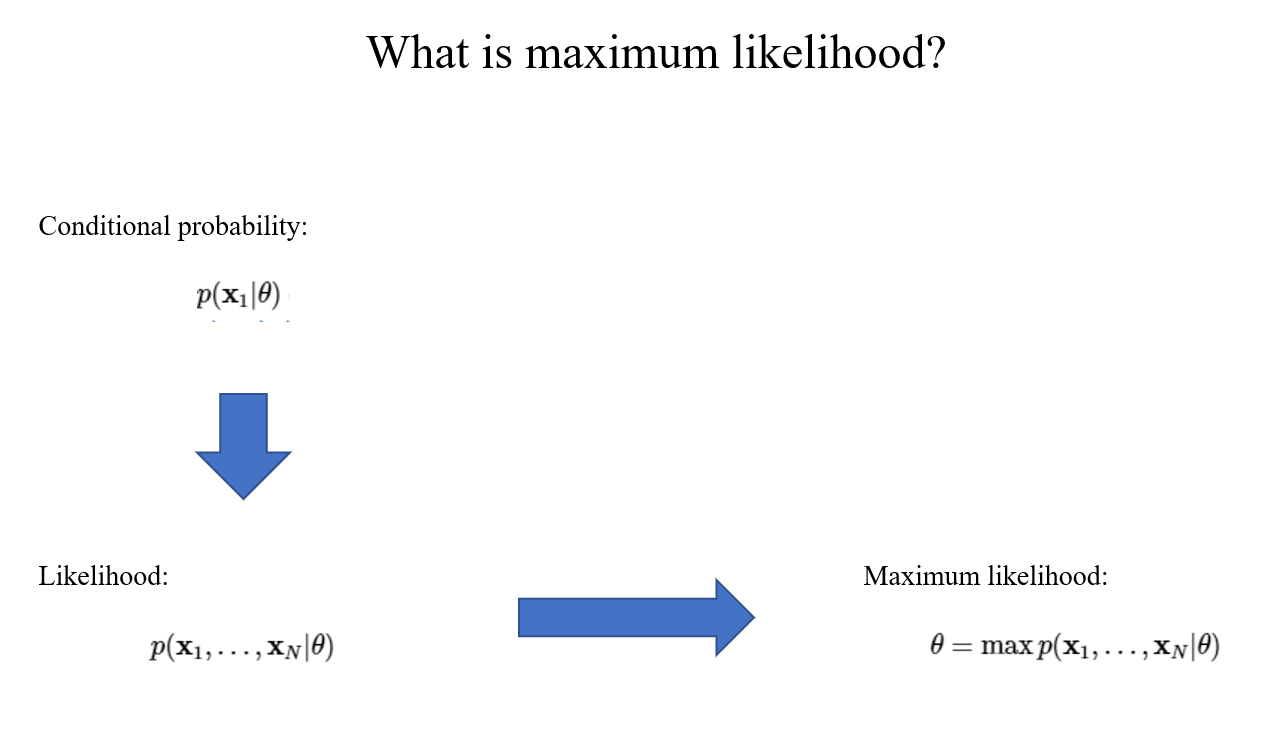
\includegraphics[scale=0.5]{Image/2.1.png}
	\caption{Tiêu chuẩn hợp lý cực đại}
	\label{fig:image2.1}
\end{figure}

Để hiểu một cách trực quan hơn ML là gì? Ta sẽ đi qua những kiến thức lý thuyết sau. Xác suất để xảy ra A khi biết B được kí hiệu là $P(A|B)$. Giả sử với bộ dữ liệu $ x_1, x_2, …, x_N $. Giả sử các điểm  $ x_1, x_2, …, x_N $ tuân theo một phân phối nào đó được mô tả bằng bộ tham số theta. Từ đây ta có khái niệm mang tên likelihood:  $ P(x_1, x_2, …, x_N | \theta) $. ML là việc tìm bộ tham số theta sao cho xác suất $ P(x_1, x_2, …, x_N | \theta) $ là lớn nhất. 

Giả sử điểm của sinh viên lớp Xác suất thống kê của Đại học Công nghệ được tuân theo phân bố chuẩn (Gaussian). Ta đã biết dữ liệu của 5 thí sinh như sau: 5, 6, 8, 2, 9. Việc ta cần làm là xác định bộ tham số độ lệch chuẩn $ \mu $ và phương sai $ \sigma $. ML sẽ được áp dụng vào bài toán như sau:
$$ P(x_i | \mu,\sigma) = \frac{1}{\sqrt{2\pi\sigma^2}} e ^ {-\frac{(x_i - \mu)^2}{2 \sigma^2}} $$

Do dữ liệu là rời rạc nên ta sử dụng ML như sau:
$$ \mu , \sigma = argmax_{\mu, \sigma} \prod_{i=1} ^ {N} P(x_i | \mu, \sigma^2) $$
$$ \Rightarrow \mu , \sigma = argmax_{\mu, \sigma} [ \frac{1}{({2\pi\sigma^2})^\frac{N}{2}} e^{\frac{-\sum_{i=1}^{N}{(x_i - \mu)}^2}{2\sigma^2}}] $$
$$ \Rightarrow \mu , \sigma = argmax_{\mu, \sigma} [-N \log{\theta} - \frac{\sum_{i=1}^{N} {(x_i - \mu)} ^ 2}{2\sigma^2}] $$

Để tìm được $\mu$ và $\sigma$, ta đạo hàm từng phần biểu thức theo $\mu$ và $\sigma$ rồi tìm giá trị của $\mu$ và $\sigma$ thỏa mãn hệ biểu thức có giá trị bằng 0. Chi tiết được tính như sau:
$$ \frac{\partial f}{\partial \mu} = \frac{1}{\sigma^2} \sum_{i=1}^{N} (x_i - \mu) = 0$$
$$ \frac{\partial f}{\partial \sigma} = -\frac{N}{\sigma} + \frac{1}{\sigma^3} \sum_{i=1}^{N} (x_i - \mu)^2 = 0$$

Giải hệ phương trình ta thu được kết quả:
$$ \mu = \frac{\sum_{i=1}^{N} x_i}{N}$$
$$ \sigma = \sqrt{\frac{\sum_{i=1}^{N} (x_i - \mu)^2}{N}}$$

Thay dữ kiện vào ta tính được kết quả như sau:
$$ \mu = 6 $$
$$ \sigma = \sqrt{6} $$

Suy luận tiến hóa bằng phương pháp maximum likelihood (ML) liên quan đến việc ước lượng các tham số của mô hình tiến hóa, độ dài cạnh trong cây và cấu trúc của cây. 

Để ước lượng cây tiến hóa theo ML cần hai bước tối ưu: tối ưu độ dài các cạnh để tính điểm cây cho mỗi cây ứng viên và duyệt tìm kiếm trong không gian cây để thu được cây làm cực đại hàm likelihood. Suy luận cây theo ML tương đương với việc so sánh nhiều giả thuyết thống kê có cùng số lượng tham số.


\section{Hệ thống phần mềm IQ-TREE}

\begin{figure}[h]
	\centering
	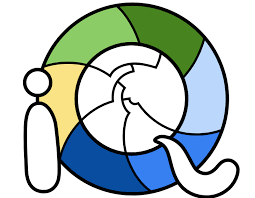
\includegraphics[scale=0.5]{Image/2.2.png}
	\caption{IQTREE}
	\label{fig:image2.2}
\end{figure}


Trong số các gói phần mềm phân tích cây tiến hóa hiện nay thì IQ-TREE là phần mềm tốt nhất (hiệu quả, chính xác). IQ-TREE được kế thừa từ chương trình TREE-PUZZLE\cite{cia-14}, khám phá không gian cây một cách hiệu quả, thường đạt được điểm likelihood cao hơn so với các phần mềm khác như RAxML và PhyML. IQ-TREE hỗ trợ các phân tích tiến hóa quan trọng (xây dựng cây tiến hóa, tính toán độ tin cậy cây tiến hóa) với miền ứng dụng phong phú của đa dạng sinh học. 

Các phương pháp tích hợp trong IQ-TREE thu hút trích dẫn lớn từ các tạp chí uy tín nhờ liên tục bổ sung các mô hình tiến hóa và cải tiến thuật toán cùng cấu trúc dữ liệu để phân tích dữ liệu cực lớn (dữ liệu hệ gen). Khả năng xử lý dữ liệu hệ gen và khả năng thực hiện ước lượng thời gian trên cây tiến hóa (mới được tích hợp) được các trung tâm nghiên cứu hàng đầu thế giới đang quan tâm sử dụng để phân tích dữ liệu coronavirus nói riêng và các virus có nguy cơ cao gây dịch nói chung (thông tin trích xuất từ IQ-TREE Google Groups \url{https://groups.google.com/d/forum/iqtree}.

Các phiên bản của gói phần mềm IQ-TREE được bắt đầu và phát triển tới nay dưới hình thức chương trình dòng lệnh. Điều này khiến việc tích hợp IQ-TREE vào các pipeline lớn khá dễ dàng và phù hợp với các nhà nghiên cứu có kinh nghiệm lập trình. Các dự án phân tích cây tiến hóa phổ biến khác như RAxML hay MrBayes đều đã có phiên bản GUI nhưng IQ-TREE thì chưa. Việc thiếu GUI khiến IQ-TREE không thân thiện với một bộ phận không nhỏ người dùng. Người dùng sẽ cần ghi nhớ khá nhiều tùy chọn tham số hay phải tra cứu từ điển hướng dẫn sử dụng để có thể thực hiện một phân tích theo nhu cầu riêng. 

Phần mềm W-IQTREE là ứng dụng trên nền web của IQ-TREE. Phiên bản này đã cố gắng khắc phục những nhược điểm của bản dòng lệnh như: đã có giao diện người dùng trực quan hơn, thân thiện hơn với người dùng, không yêu cầu người dùng có kiến thức về dòng lệnh để thực hiện phân tích hay giảm thiểu được thời gian và công sức phải ghi nhớ lệnh. Tuy nhiên, W-IQTREE thiếu tương tác trực quan với cây tiến hóa và khi có quá nhiều lượng truy cập để thực hiện phân tích kiểm định thống kê thì sẽ có hiện tượng thắt nút cổ chai làm ảnh hưởng trải nghiệm của người dùng hay hiệu năng của hệ thống. Hơn nữa, người dùng e ngại về tính cá nhân hóa và bảo mật dữ liệu của họ vì phải đẩy dữ liệu lên Internet.

Trong khóa luận này, em thực hiện nghiên cứu các giải pháp và phát triển thành công phần backend cho phần mềm ứng dụng desktop GIQ-TREE (/gig tri:/) đáp ứng các mục tiêu nói trên. Việc thành công của ứng dụng RAxML GUI2.0 so với phiên bản tiền nhiệm RAxML GUI(2011) đã làm cho em chắc chắn hơn về luận điểm một ứng dụng desktop với dữ liệu mang tính cá nhân hóa của người dùng. Phiên bản GIQ-TREE có khả năng khắc phục được vấn đề thắt nút cổ chai của phiên bản tiền nhiệm W-IQTREE cũng như mang lại tính cá nhân hóa dữ liệu cho người dùng khiến trải nghiệm người dùng được cải thiện. Phần mềm được cung cấp miễn phí và được đưa ra dưới dạng mã nguồn mở để cộng đồng có thể cùng thảo luận và đóng góp.

\subsection{Mô hình tiến hóa cho dữ liệu đơn gen}
Suy luận tiến hóa theo tiêu chuẩn ML được gọi là suy luận tiến hóa dựa trên mô hình bởi nó cần mô hình tiến hóa để tính điểm số của cây. Mô hình tiến hóa là một tập các giả định về quá trình biến đổi nucleotide hay axít amin. Nó cho biết các xác suất để biến đổi từ trạng thái này sang trạng thái khác dọc theo một cây tiến hóa.

IQ-TREE hỗ trợ hầu hết các mô hình biến đổi phổ biến trong tin sinh cho nhiều loại dữ liệu khác nhau: DNA, protein, codon, nhị phân và cả dữ liệu hình thái. Ngoài ra, IQ-TREE cũng có khả năng tính toán theo các mô hình có tính tới tốc độ biến thiên giữa các vị trí trong chuỗi như Gamma hay FreeRate. Nhờ vậy, nó mô hình hóa thành công dữ liệu thực trong nhiều công trình trích dẫn.

Trường hợp người dùng không có thông tin về mô hình tiến hóa của dữ liệu cần phân tích, IQ-TREE sử dụng những cách tiếp cận được chấp nhận rộng rãi để đề xuất mô hình phù hợp nhất dựa trên likelihood hoặc các độ đo theo lý thuyết thông tin.
\subsection{Mô hình tiến hóa cho dữ liệu đa gen}
Trong suy luận tiến hóa hệ gen (đầu vào là một sắp hàng hệ gen), người ta thường cho phép mỗi phân hoạch (mỗi gen) có mô hình tiến hóa riêng.

Nhờ cài đặt tính toán hiệu quả ở phần lõi, IQ-TREE có khả năng phân tích dữ liệu lớn và hỗ trợ nhiều mô hình đa gen tiên tiến. Với phân tích nhiều gen, người dùng chỉ cần cung cấp một tệp phân hoạch (như trong IQ-TREE) hoặc một thư mục của các sắp hàng đơn gen (IQ-TREE).
\subsection{Các kiểm định thống kê đánh giá cây tiến hóa}
Cây tốt nhất tìm được bởi một thuật toán tìm cây có vai trò như một ước lượng tham số. Do đó, phân tích đầy đủ cần kèm theo đánh giá đỗ hỗ trợ thống kê thông qua các phương pháp kiểm định thống kê khác nhau. Để kiểm tra độ tin cậy của các cạnh trong một cây nhất định, ta có thể sử dụng bootstrapping (phi tham số) để tính giá trị hỗ trợ trên các cạnh. Ngoài ra, có những kiểm định giúp so sánh các cấu trúc cây không lồng nhau và mâu thuẫn có khoảng cách tương đương tới cây đúng hay không .
\subsection{Suy luận thời gian trên cây tiến hóa}
Suy luận thời gian diễn ra các sự kiện tiến hóa (các đỉnh trong của cây) là bài toán được quan tâm, đặc biệt với dữ liệu của virus. Để thực hiện suy luận, bài toán cần thêm thông tin thời gian, hoặc cho ở nút lá, hoặc ở đỉnh trong. IQ-TREE2 tích hợp thuật toán LSD2 \cite{cia-15} là một thuật toán có khả năng suy luận thời gian hiệu quả trên dữ liệu lớn.

\newpage	
\chapter{Phân tích các yêu cầu và công nghệ sử dụng}
\label{chap:chapter3}

\section{Phân tích các yêu cầu}
\subsection{Yêu cầu chức năng}
Các yêu cầu chức năng được liệt kê như sau:

- Cài đặt các chức năng đã có của bản website và chuyển đổi thành các chức năng trên ứng dụng desktop

- Ánh xạ cài đặt các mẫu yêu cầu từ bản command-line sang thành các chức năng trên ứng dụng desktop

- Quản lý cấu trúc dự án và các vấn đề liên quan đến hệ thống tệp (file system)

- Quản lý cấu trúc và các vấn đề liên quan đến tiến trình
\subsection{Yêu cầu phi chức năng}
Các yêu cầu phi chức năng được liệt kê như sau:

- Tính khả mở rộng

- Đáp ứng chịu tải tốt, tính riêng tư dữ liệu

- Rút gọn dung lượng cần thiết

- Ứng dụng có thể chạy trên mọi nền tảng thông dụng hiện nay

\section{Các cơ chế phát triển web}
\subsection{Server-side rendering}
Các trang web sử dụng cơ chế này: toàn bộ các CMS như Joomla, WordPress. Các trang web ở Việt Nam: Thegioididong, Vnexpress, Zing News, …

\begin{figure}[h]
	\centering
	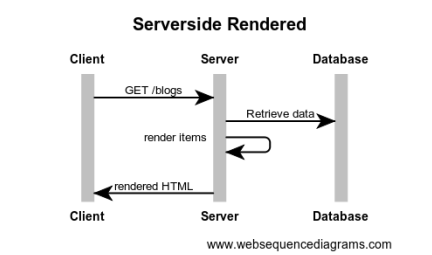
\includegraphics[scale=1.2]{Image/3.1.png}
	\caption{Server-side rendering (nguồn websequencediagrams.com) }
	\label{fig:image3.1}
\end{figure}

Cơ chế này có phần lớn logic được xử lý ở máy chủ (server). Khi người dùng vào một trang web, trình duyệt sẽ gửi yêu cầu lên máy chủ web (ví dụ với phương thức GET). Sau đó, máy chủ web sẽ nhận yêu cầu và thực hiện các logic để lấy dữ liệu từ cơ sở dữ liệu (database). Tiếp theo, máy chủ web sẽ kết xuất HTML và trả về các tệp HTML cho người dùng.

Ưu điểm:

- Phía máy khách (client) chỉ việc hiển thị vì tất cả dữ liệu đã được xử lý ở máy chủ (server

- Các web framework từ trước đến nay đều có hỗ trợ cơ chế này (lấy đơn cử Node.js cũng có các engine như pug hay ejs hỗ trợ việc này)

- Dễ hiểu và dễ phát triển những dòng lệnh hơn vì lập trình viên chỉ cần phát triển một dự án web là được, không cần thiết phải tách ra làm hai phần front-end và back-end

- SEO tốt vì khi bot của các trang tìm kiếm như Google, Bing vào web sẽ thấy toàn bộ dữ liệu HTML

- Chạy được phần lớn trên mọi trình duyệt ngay cả khi ngắt JavaScript

Nhược điểm:

- Tương tác không tốt như client-side rendering vì mỗi lần người dùng chuyển trang là phải tải dữ liệu lại nhiều lần, gây ra trải nghiệm người dùng không cao

- Tốn tài nguyên ở máy chủ (server) vì máy chủ phải xử lý nhiều logic và dữ liệu (có thể dùng cơ chế caching để giảm tải)

\subsection{Client-side rendering}
Với việc công nghệ phát triển mạnh mẽ và nhiều biến thể để giải quyết các vấn đề gặp phải, sự phát triển của JavaScript và AJAX vào những năm 2010 kèm theo sự phát triển phần cứng của các máy tính cá nhân đã làm cơ chế client-side rendering bắt đầu được sử dụng. Những trang web sử dụng cơ chế này có thể kể đến như: Facebook (React), Instagram(React), Netflix (React), Trello (Angular), Gitlab (VueJS), …

\begin{figure}[h]
	\centering
	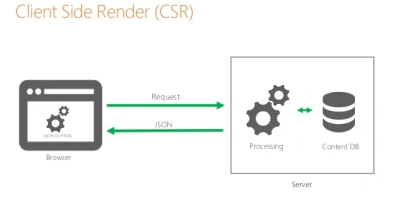
\includegraphics[scale=1]{Image/3.2.png}
	\caption{Client-side rendering (nguồn toidicodedao.com) }
	\label{fig:image3.2}
\end{figure}

Các lập trình viên bắt đầu xây dựng ứng dụng dưới dạng SPA. Client-side rendering tức việc kết xuất HTML, CSS sẽ được thực hiện ở bên máy khách (client) thay vì máy chủ(server) như server-side rendering. Các phần logic về hiển thị sẽ được thực thi tại bên máy khách (client), còn các logic quan trọng và phức tạp vẫn sẽ thực hiện bên máy chủ (server).

Ưu điểm:

- Trang chỉ cần tải một lần duy nhất. Khi người dùng chuyển trang hoặc thêm dữ liệu (lọc, sắp xếp, …) thì JavaScript sẽ lấy dữ liệu từ máy chủ (server) thông qua AJAX khiến người dùng có thể thấy dữ liệu mới mà không cần chuyển trang

- Giảm tải cho máy chủ (server) về xử lý logic

- Giảm được băng thông đường truyền mạng do chỉ cần lấy JSON là dữ liệu cần thiết thay vì lấy toàn bộ trang.

- Tốt với các ứng dụng tương tác nhiều, bởi vì SPA hoạt động tốt hơn khi dòng lệnh chạy trên trình duyệt, không cần tải đi tải lại nhiều lần.

Nhược điểm:

- Ứng dụng có thể chạy chậm nếu không biết tối ưu. Lý do là trình duyệt cần xử lý một phần dữ liệu sau đó mới kết xuất.

- Đòi hỏi dự án cần chia làm hai phần riêng là back-end và front-end, do đó phát triển khó hơn

- Không chạy được nếu JavaScript ở trình duyệt bị tắt hoặc các trình duyệt cũ không nhận JavaScript ES6.

- SEO không tốt bằng server-side rendering do bot khó đọc dữ liệu.

- Nếu máy khách có phần cứng yếu thì việc tải trang sẽ rất chậm.

Cả hai cơ chế đều được sử dụng rộng rãi tùy vào bài toán cụ thể mà sẽ cần áp dụng cơ chế server-side rendering hay client-side rendering. Trước khi phát triển, lập trình viên cần hiểu rõ các ưu và nhược điểm của mỗi cơ chế và phân tích bài toán để tìm cơ chế phù hợp để áp dụng. GIQ-TREE đã được xây dựng dựa trên cơ chế dựa trên sự tham khảo của cơ chế client-side rendering nhằm tách riêng hai thành phần back-end và front-end ra cũng như hai phần tương tác với nhau thông qua các sự kiện bằng dữ liệu JSON.

\section{Các công nghệ, công cụ áp dụng trong khóa luận}
\subsection{Node.js}
Node.js là một hệ thống phần mềm được thiết kế để viết các ứng dụng internet có khả năng mở rộng, đặc biệt là máy chủ web. Chương trình được viết bằng JavaScript, sử dụng kỹ thuật điều khiển theo sự kiện, nhập/xuất không đồng bộ để tối thiểu tổng chi phí và tối đa khả năng mở rộng. Node.js bao gồm có V8 JavaScript engine của Google, libUV, và vài thư viện khác.

Node.js được tạo bởi Ryan Dahl từ năm 2009, và phát triển dưới sự bảo trợ của Joyent.
Mục tiêu ban đầu của Dahl là làm cho trang web có khả năng push như trong một số ứng dụng web như Gmail. Sau khi thử với vài ngôn ngữ Dahl chọn Javascript vì một API Nhập/Xuất không đầy đủ. Điều này cho phép anh có thể định nghĩa một quy ước Nhập/Xuất điểu khiển theo sự kiện, non-blocking.

Vài môi trường tương tự được viết trong các ngôn ngữ khác bao gồm Twisted cho Python, Perl Object Environment cho Perl, libevent cho C và EventMachine cho Ruby. Khác với hầu hết các chương trình Javascript, Nodejs không chạy trên một trình duyệt mà chạy trên Server. Node.js sử dụng nhiều chi tiết kỹ thuật của CommonJS. Nó cung cấp một môi trường REPL cho kiểm thử tương tác. Node.js được InfoWorld bình chọn là "Công nghệ của năm" năm 2012
\subsection{Electron.js}
Electron (trước đây gọi là Atom Shell) là một phần mềm mã nguồn mở và miễn phí được phát triển và duy trì bởi GitHub. Nó cho phép phát triển các ứng dụng GUI trên máy tính để bàn sử dụng công nghệ web: nó kết hợp công cụ kết xuất Chromium và Node.js run time. Electron là khung GUI chính đằng sau một số dự án mã nguồn mở bao gồm Atom, GitHub Desktop, Light Table, Visual Studio Code, Evernote, và WordPress Desktop.

Electron.js bao gồm nhiều tiến trình. Nó sẽ có tiến trình chính (main process) và các trình kết xuất (renderer processes). Tiến trình chính chạy logic của ứng dụng và có thể khởi chạy nhiều các trình kết xuất khác nhau được hiển thị bằng cách biên dịch mã nguồn HTML, CSS tương ứng. Cả hai dạng tiến trình đều có thể tích hợp với Node.js.
Tuy nhiên, để đánh đổi lại sự tiện lợi và dễ phát triển, Electron có thể chiếm nhiều dung lượng RAM hơn các ứng dụng tương tự được xây dựng với các công nghệ nguồn gốc từ hệ điều hành (native applications)
\subsection{SQLite}
SQLite được Richard Hipp viết dưới dạng thư viện bằng ngôn ngữ lập trình C. SQLite là hệ thống cơ sở dữ liệu quan hệ nhỏ gọn, hoàn chỉnh, có thể cài đặt bên trong các trình ứng dụng khác. Các điểm sáng trong SQLite bao gồm: (i) Tin cậy: các hoạt động trong cở dữ liệu được thực hiện trọn vẹn, rất hiếm khi gây lỗi sự cố phần cứng. (ii) Tuân theo chuẩn SQL92 (chỉ một vài đặc điểm không được hỗ trợ) (iii) Không cần cài đặt cấu hình (iv) Kích thước gọn nhẹ với cấu hình đầy đủ cho các tác vụ cơ bản (v) Không cần cài đặt phần mềm phụ trợ đi kèm
\subsection{Azure Devops}
Azure DevOps Server (trước đây là Team Foundation Server (TFS) và Visual Studio Team System (VSTS)) là một sản phẩm của Microsoft cung cấp kiểm soát phiên bản (với Team Foundation Version Control (TFVC) hoặc Git), báo cáo, quản lý yêu cầu, quản lý dự án ( cho cả nhóm phát triển phần mềm nhanh nhẹn và nhóm thác nước), khả năng quản lý xây dựng, thử nghiệm và phát hành tự động. Nó bao gồm toàn bộ vòng đời ứng dụng và cho phép các khả năng của DevOps. Azure DevOps có thể được sử dụng như một phần mềm hỗ trợ cho nhiều môi trường phát triển tích hợp (IDE) nhưng được thiết kế riêng cho Microsoft Visual Studio và Eclipse trên tất cả các nền tảng. 
\subsection{Git}
Hiện nay, Git là một công cụ hỗ trợ cho các lập trình viên rất nhiều trong việc theo dõi và lưu trữ lịch sử của các dòng lệnh. Git là phần mềm quản lý mã nguồn phân tán được phát triển bởi Linus Torvalds vào năm 2005, ban đầu dành cho việc phát triển nhân Linux. Hiện nay, Git trở thành một trong các phần mềm quản lý mã nguồn phổ biến nhất. Git là phần mềm mã nguồn mở được phân phối theo giấy phép công cộng GPL2.
\subsection{Diagrams.net}
Diagrams.net trước đây có tên gọi là draw.io là một phần mềm mã nguồn mở đa nền tảng được phát triển dựa trên HTML và JavaScript. Với Diagrams.net, người dùng có thể tạo các sơ đồ (diagrams) như luồng điều khiển (flowcharts), wireframes, sơ đồ UML, sơ đồ mạng, …

Diagrams.net khả dụng trên các nền tảng trình duyệt trực tuyến và phần mềm ứng dụng tương thích trên các hệ điều hành khác nhau như Windows, Linux, MacOS. Phần mềm ứng dụng của Diagrams.net được phát triển bằng Electron framework. Phần mềm không yêu cầu có tài khoản để đăng nhập và có thể lưu dữ liệu ngay trên ổ cứng của thiết bị máy tính cá nhân của người dùng.

Phần mềm hỗ trợ việc xuất các tệp có định dạng như PNG, JPEG, SVG, PDF.

Chưa dừng ở đó, Diagrams.net còn có thể tích hợp với các ứng dụng lưu trữ điện toán đám mây khác như Dropbox, OneDrive, Google Drive, Github hay Gitlab. Việc này hỗ trợ rất nhiều cho các nhóm phát triển sản phẩm, giúp tối ưu hóa thời gian và hiệu suất làm việc.

Diagrams.net còn tích hợp dưới dạng plugin cho phép nhúng vào các phần mềm web trên các nền tảng như NextCloud, MediaWiki, Notion (một phần mềm rất thu hút hiện nay), Confluence (phần mềm các doanh nghiệp sử dụng để lưu trữ và chia sẻ các tài liệu về các dự án) hay Jira (một phần mềm giúp việc quản lý dự án dễ dàng và hiệu suất hơn)

\newpage	
\chapter{Xây dựng back-end cho hệ thống GUI}
\label{chap:chapter4}
\section{Tổng quan hệ thống}
Sau khi phân tích các yêu cầu cũng như tìm hiểu về các công nghệ áp dụng. Sau đây, em xin được đưa ra giải pháp thiết kế cho phần back-end của ứng dụng GIQ-TREE.

Với các yêu cầu chức năng đưa ra, em xin đưa ra yêu cầu thiết kế như sau:

- Cài đặt các chức năng đã có của bản website: Dùng thử bản website và hình dung các luồng làm việc và khởi chạy dữ liệu cũng như tạo ra các bản nháp để thiết kế hệ thống. Cài đặt và tích hợp (rất nhiều) tính năng của bản website lên trên bản desktop. Ánh xạ cài đặt của bản desktop. Nhận yêu cầu từ bảng tra cứu để thực hiện ánh xạ các cài đặt cần thiết cho ứng dụng.

- Quản lý cấu trúc dự án và các vấn đề liên quan đến hệ thống tệp (file system): Sử dụng nền tảng Node.js với các hỗ trợ về hệ thống tệp kèm theo để quản lý hệ thống tệp (file system) của máy tính. Sử dụng framework Electron.js để hỗ trợ việc thực hiện các popup nhận các dữ liệu khởi tạo dự án hay nhập các tệp đầu vào của dự án cũng như mở lại các dự án đã được tạo. Sử dụng sqlite3 với những ưu điểm là dung lượng nhỏ và tối giản những thứ vừa đủ cho dự án. Sử dụng cơ sở dữ liệu như là một bảng tra cứu (lookup table) với mỗi định danh như là một con trỏ lưu địa chỉ và giá trị của dự án được khởi tạo

- Quản lý cấu trúc và các vấn đề liên quan đến tiến trình: Sử dụng các module như process, child-process để quản lý các tiến trình được khởi tạo và chạy cũng như các signal để giết các tiến trình cũng như bắt đầu lại. Việc chọn signal đã được tác giả của IQTREE bản command-line viết trong mã nguồn bằng ngôn ngữ C, chi tiết sẽ được làm rõ khi đọc mã nguồn mở đó.

Với các yêu cầu phi chức năng đưa ra, em xin đưa ra yêu cầu thiết kế như sau:

- Tính khả mở rộng: Có khả năng mở rộng sau này bằng cách chèn các vùng, bảng tra cứu thêm vào khi đã áp dụng cơ sở dữ liệu để lưu trữ

- Đáp ứng chịu tải tốt, tính riêng tư dữ liệu: Do không bị ràng buộc bởi các vấn đề liên quan như kết nối mạng internet hay lưu trữ trên đám mây (cloud) nên sẽ đảm bảo tính riêng tư dữ liệu của người dùng

- Rút gọn dung lượng cần thiết: Rút gọn vấn đề tải cả phiên bản gốc của iqtree ngay trong ứng dụng bằng cách tự động tải và giải nén phiên bản lõi của IQTREE sau khi đã cài đặt xong ứng dụng

- Ứng dụng có thể chạy trên mọi nền tảng thông dụng hiện nay: Như đã nói, ứng dụng được dựng nên từ Electron.js sau đó sẽ dựng nên các bản ứng dụng cho từng nền tảng nên có thể chạy ổn định trên các nền tảng hệ điều hành thông dụng ngày nay như Windows, Linux hay MacOS
\subsection{Ca sử dụng của hệ thống}
Ca sử dụng (use case) là một khái niệm quen thuộc và quan trọng trong phát triển phần mềm. Ca sử dụng như là một chuỗi các hành động được hệ thống thực hiện và mang lại kết quả quan sát được của giá trị cho một tác nhân cụ thể. Ca sử dụng mô tả sự tương tác đặc trưng giữa người dùng bên ngoài và hệ thống. Đơn giản có thể hiểu ca sử dụng là một kỹ thuật được dùng trong kỹ thuật phần mềm và hệ thống để nắm bắt yêu cầu chức năng của hệ thống. Trong ca sử dụng, có hai thành phần cần quan tâm là tác nhân (actors) và các hành động. \textbf{Hình \ref{fig:image4.1}} thể hiện về ca sử dụng của người dùng trong hệ thống GIQ-TREE. Người dùng có thể khởi tạo dự án, quản lý dự án, xem các dự án đã được tạo hay tra cứu dự án đã được tạo theo tên. Chưa dừng ở đó, người dùng còn có thể xem được các dữ liệu văn bản thô của dữ liệu đầu vào, đầu ra để kiểm tra tính đúng đắn của dữ liệu. Ở phần cài đặt các phân tích kiểm định thống kê, người dùng có thể thay đổi các cài đặt dựa trên các ràng buộc về dữ liệu. Sau khi hoàn thành tinh chỉnh người dùng có thể lưu lại và thực hiện các phân tích cũng như tạm dừng hay tiếp tục phân tích. Kết quả đầu ra sẽ được hiển thị dưới dạng giao diện người dùng.

\begin{figure}[h]
	\centering
	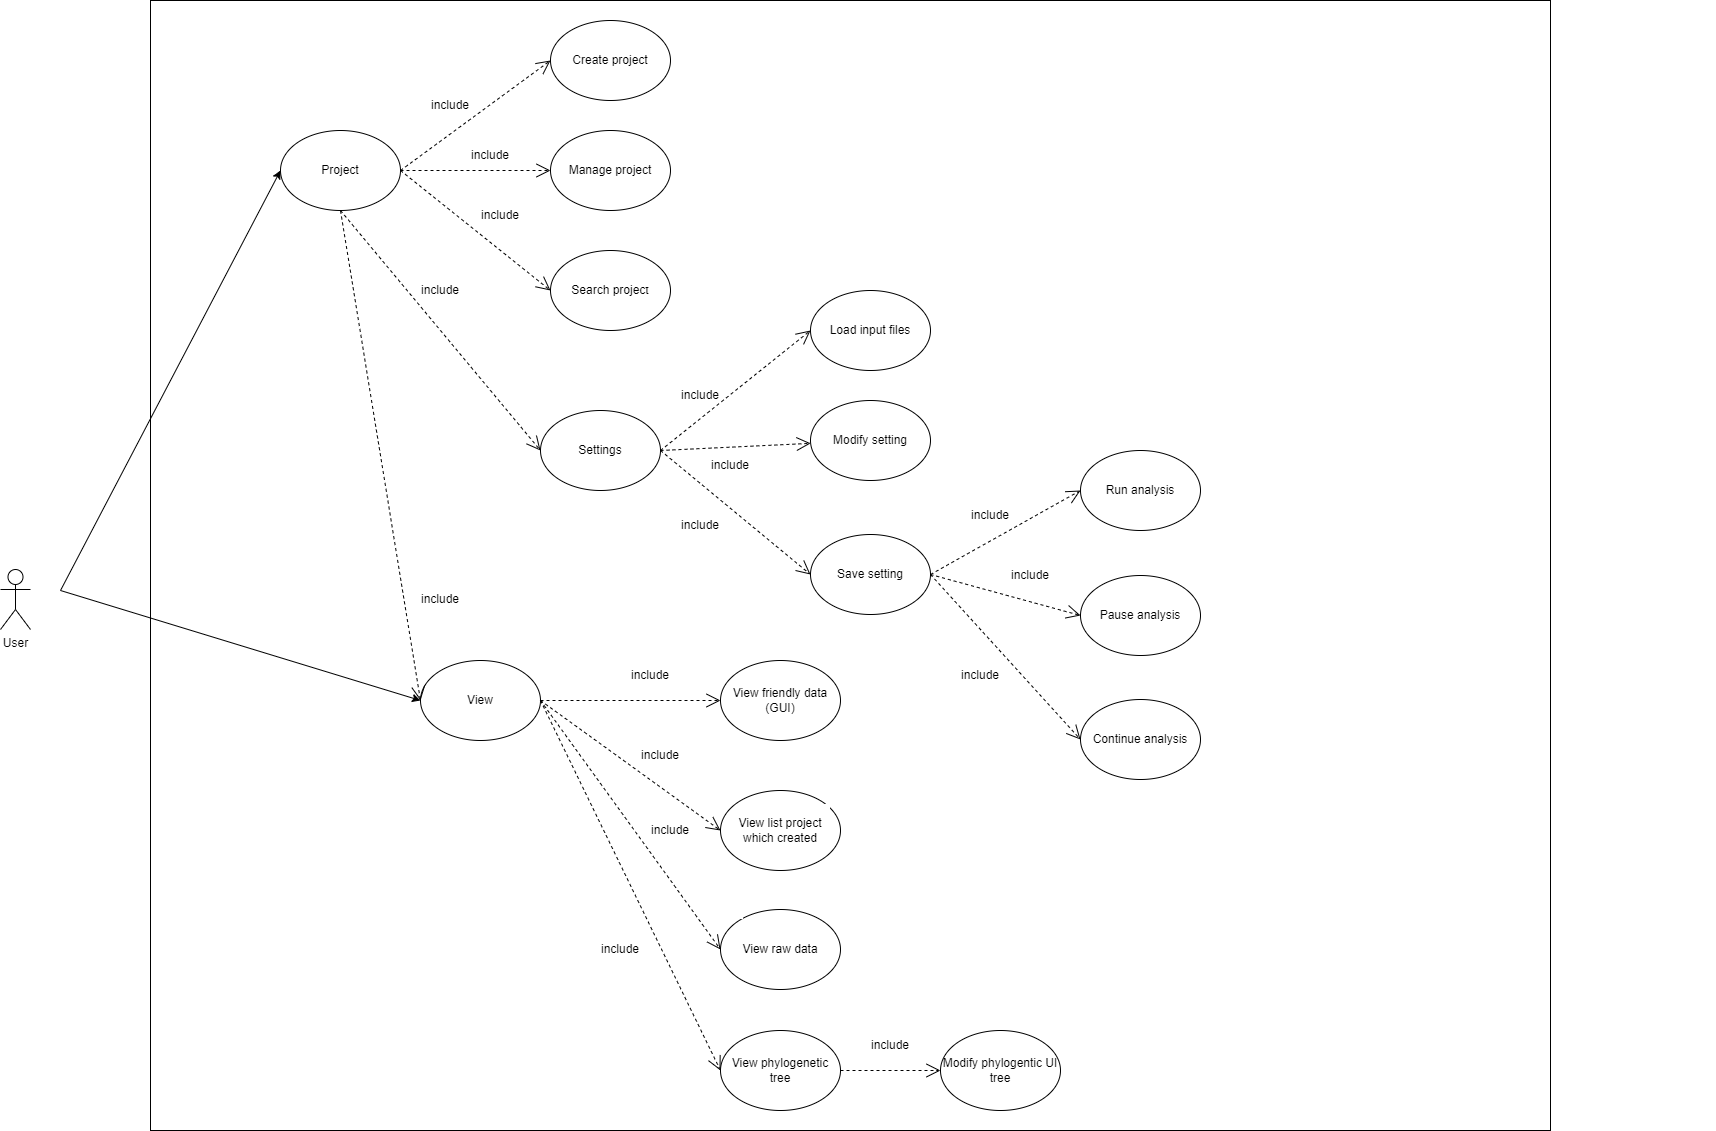
\includegraphics[scale=0.3]{Image/4.1.png}
	\caption{Hình ảnh ca sử dụng cho người dùng của hệ thống GIQ-TREE }
	\label{fig:image4.1}
\end{figure}

\subsection{Luồng điều khiển của ứng dụng}
Trước khi khởi chạy ứng dụng, cần có bước nhúng và cài đặt ứng dụng IQTREE một cách tự động. Đầu tiên, ứng dụng GIQ-TREE sẽ kiểm tra hệ điều hành trên máy tính cá nhân người dùng đang sử dụng là hệ điều hành gì để có thể kiểm tra cần cài đặt phiên bản IQTREE nào cho máy tính người dùng. Tiếp theo ứng dụng sẽ kiểm tra xem IQTREE đã có sẵn phiên bản đó trên máy tính người dùng hay chưa (tại đường dẫn trên máy tính)? Từ đó đưa ra quyết định là có tải ứng dụng IQTREE về và giải nén trên máy tính của họ hay không? Kết thúc bước trên, ứng dụng tiếp tục kiểm tra xem cơ sở dữ liệu về GIQ-TREE đã có trên máy tính người dùng hay chưa để khởi tạo cơ sở dữ liệu nhằm mục đích lưu trữ dữ liệu cũng như thuận lợi trong quá trình mở rộng ứng dụng sau này. Kết thúc các bước thì ứng dụng GIQ-TREE sẽ được khởi chạy. Chi tiết các bước kể trên có thể thấy ở c\textbf{Hình \ref{fig:image4.2}}

\begin{figure}[h]
	\centering
	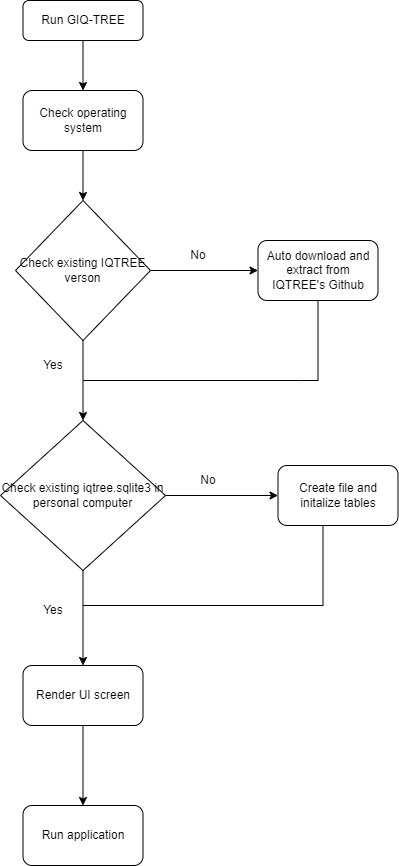
\includegraphics[scale=0.65]{Image/4.2.png}
	\caption{Sơ đồ thể hiện việc nhúng IQTREE vào bên trong GIQ-TREE và khởi tạo cơ sở dữ liệu }
	\label{fig:image4.2}
\end{figure}

\subsection{Cơ sở dữ liệu lưu trữ tối giản của ứng dụng}
Cơ sở dữ liệu là một phần không thể thiếu của các dự án phần mềm. Nó giúp phần lưu trữ dữ liệu theo quan hệ hoặc phi quan hệ với các mục đích riêng biệt như làm tăng hiệu năng của hệ thống, giảm chi phí phát triển và mở rộng hệ thống hay chỉ đơn giản là tách riêng dữ liệu lưu trữ ra khỏi các phần “động” khác. Phần mềm GIQ-TREE đã tối ưu bằng cách chỉ có ba bảng như sau trong cơ sở dữ liệu: 

- Bảng project thể hiện các dự án của GIQ-TREE mà người dùng khởi tạo, gồm các trường như:(i) project\textunderscore id  để thể hiện định danh của dự án,(ii) name để thể hiện tên của dự án,(iii) time để thể hiện thời điểm khởi tạo dự án,(iv) process để thể hiện trạng thái tiến trình của dự án, (v)path để thể hiện đường dẫn của dự án , (vi)project\textunderscore type để thể hiện kiểu của dự án.

- Bảng input thể hiện các dữ liệu đầu vào bao gồm các trường: (i)input\textunderscore id thể hiện định danh của dữ liệu đầu vào (ii) name để thể hiện tên dữ liệu đầu vào (iii) path để thể hiện đường dẫn của dữ liệu đầu vào (iv) project\textunderscore id để thể hiện định danh của dự án mà dữ liệu này nằm trong.

- Bảng output thể hiện các dữ liệu đầu ra bao gồm các trường: (i) output\textunderscore id thể hiện định danh của dữ liệu đầu ra (ii) name để thể hiện tên dữ liệu đầu ra (iii) path để thể hiện đường dẫn của dữ liệu đầu ra (iv) project\textunderscore id để thể hiện định danh của dự án mà dữ liệu này nằm trong.

Chi tiết đã được mô tả trong \textbf{Hình \ref{fig:image4.3}}

\begin{figure}[h]
	\centering
	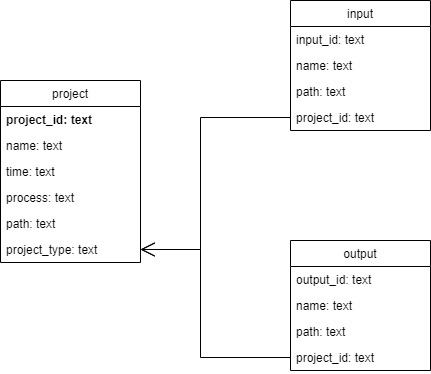
\includegraphics[scale=1]{Image/4.3.png}
	\caption{Hình ảnh thể hiện mối liên kết các bảng trong cơ sở dữ liệu }
	\label{fig:image4.3}
\end{figure}

Do GIQ-TREE là ứng dụng chạy trên máy tính người dùng nên dự án này lựa chọn cách lưu trữ dữ liệu dựa trên hệ quản trị cơ sở dữ liệu mang tên SQLite3 nhằm tối ưu dung lượng cũng như lược bỏ các cài đặt không cần thiết. Câu hỏi đặt ra là tại sao cần đặt vào hệ quản trị cơ sở dữ liệu mà không lưu trữ dưới dạng khác như các tệp đơn thuần? Việc tích hợp hệ quản trị cơ sở dữ liệu vào nhằm mục đích tăng khả năng mở rộng cho ứng dụng về sau này. Ứng dụng hướng đến mục tiêu chạy lâu dài và ổn định chứ không đơn thuần là bản chạy một lần.

\section{Cách tổ chức tệp lưu trữ dữ liệu dự án của ứng dụng }
Cấu trúc thư mục của IQTREE nhìn qua rất rối rắm và phi logic \textbf{Hình \ref{fig:image4.4}} và phụ thuộc rất nhiều vào cách người dùng phải bố trí thư mục sao cho hợp lý. Tính chất này có thể coi như là ưu điểm với những người dùng đòi hỏi tính cá nhân hóa cao khi họ muốn tự tay làm hết tất cả nhưng lại nhược điểm khi làm mất thời gian của người dùng trong cách bố trí và sắp xếp thư mục. Chính vì thế, để tiết kiệm thời gian cho người dùng về việc sắp xếp cũng như lưu trữ dữ liệu. GIQ-TREE đưa ra việc lưu trữ với mỗi dự án như \textbf{Hình \ref{fig:image4.5}, Hình \ref{fig:image4.6}} 

- Thư mục input: chứa các tệp hay thư mục thể hiện dữ liệu đầu vào

- Thư mục output: chứa các tệp hay thư mục thể hiện dữ liệu đầu ra

- Tệp setting.json thể hiện các tinh chỉnh cài đặt của dữ liệu mỗi dự án

Chi tiết xem tại hình bên dưới:

\begin{figure}[h]
	\centering
	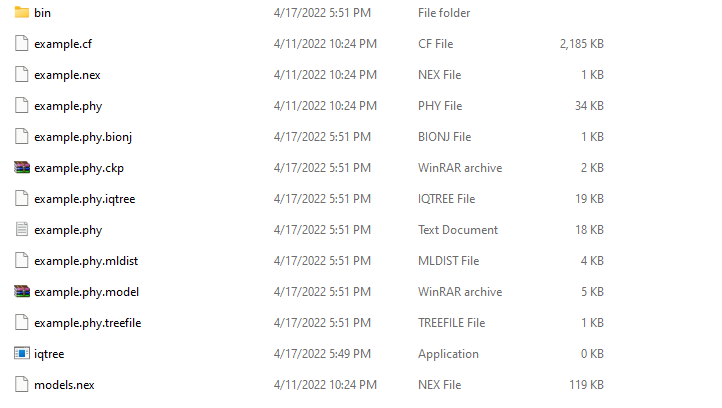
\includegraphics[scale=1]{Image/4.4.png}
	\caption{Cấu trúc thư mục của một dự án trong IQTREE }
	\label{fig:image4.4}
\end{figure}

\begin{figure}[h]
	\centering
	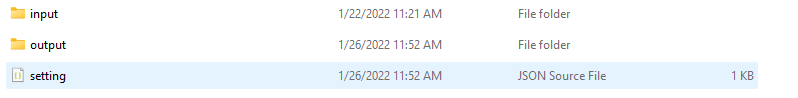
\includegraphics[scale=1]{Image/4.5.png}
	\caption{Cấu trúc thư mục của mỗi dự án trong GIQ-TREE }
	\label{fig:image4.5}
\end{figure}

\begin{figure}[h]
	\centering
	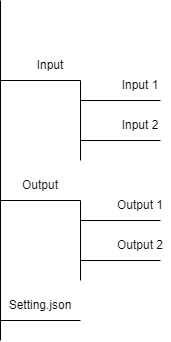
\includegraphics[scale=1]{Image/4.6.png}
	\caption{Cấu trúc thư mục của mỗi dự án trong GIQ-TREE }
	\label{fig:image4.6}
\end{figure}

\subsection{Chi tiết cài đặt}
Việc phát triển thiết kế phân cấp trực quan cho các tùy biến nhằm khắc phục điểm yếu của bản dòng lệnh là có nhiều đối số khiến người dùng phổ thông khó nhớ hết( \textbf{Hình \ref{fig:image4.7}}). Thiết kế dựa trên việc kết quả thống kê các thẻ chủ đề thường đi cùng nhau qua phân tích dữ liệu IQTREE Google Groups và việc nhóm chương trong từ điển hướng dẫn sử dụng. Các tùy biến trong GIQ-TREE được chia vào 6 nhóm chính là: Data, Model, Tree Search, Assessment, Dating, Others. Chi tiết được thể hiện trong  \textbf{
Bảng\ref{tbl:table4.1}}

\begin{figure}[h]
	\centering
	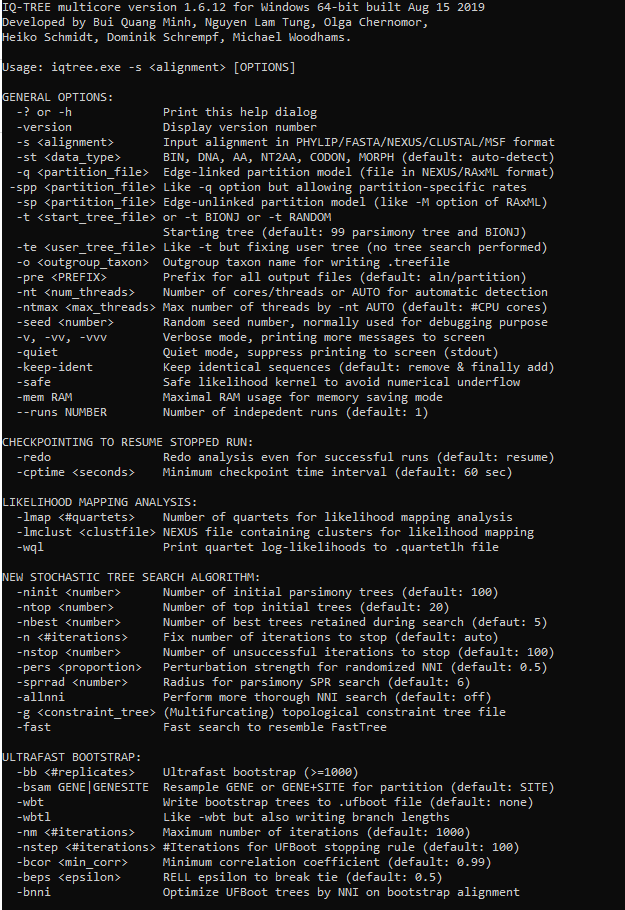
\includegraphics[scale=0.8]{Image/4.7.png}
	\caption{Tùy chọn cài đặt của IQTREE }
	\label{fig:image4.7}
\end{figure}

\begin{longtable}[c]{|p{2.5cm}|p{6.5cm}|p{6.5cm}|}
\caption{Đề xuất phân cấp trực quan cho các tùy biến dòng lệnh}
\label{tbl:table4.1}
\hline
\textbf{Nhóm} & \textbf{Tùy biến} & \textbf{Giải thích} \\
\endfirsthead
%
\endhead
%
\hline
		\textbf{Data}              & Alignment file(s)/folder*        &        Chọn tệp/thư mục dữ liệu vào                          \\ \hline
		\textbf{Data}             & Partition file     &            Chọn tệp phân hoạch             \\ \hline
		\textbf{Data}           & Sequence type    &            Chỉ định loại dữ liệu                      \\ \hline
		\textbf{Data}              & Partition type        &        Chỉ định loại phân hoạch                         \\ \hline
		\textbf{Model}             & Substitution model    &            Chỉ định mô hình biến đổi            \\ \hline
		\textbf{Model}           & Rate heterogeneity across sites   &            Chỉ định mô hình biến thiên tốc độ giữa các cột                     \\ \hline
		\textbf{Model}              & State frequency        &        Chỉ định mô hình tần suất trạng thái                      \\ \hline
		\textbf{Model}             & Ascertainment bias correction    &            Chỉ định việc chỉnh sửa bias            \\ \hline
		\textbf{Model}           & Auto-merge partitions   &            Tùy chọn bật tự động ghép phân hoạch                     \\ \hline
		\textbf{Model}              & Merging algorithm        &        Thuật toán tự động ghép phân hoạch                          \\ \hline
		\textbf{Tree Search}             & On    &            Tùy chọn bật tìm kiếm cây             \\ \hline
		\textbf{Tree Search}           & Number of unsuccessful iterations to stop    &            Chỉ định điều kiện dừng                      \\ \hline
		\textbf{Tree Search}              & Perturbation strength (between 0 and 1) for randomized NNI       &        Chỉ định mức độ phá cây khi làm tìm kiếm                          \\ \hline
		\textbf{Tree Search}             & Constrained tree file    &            Chỉ định cây khung            \\ \hline
		\textbf{Tree Search}           & Reference tree    &            Chỉ định cây tham chiếu                     \\ \hline
		\textbf{Assessment}              & Bootstrap method       &        Chỉ định phương pháp bootstrap                         \\ \hline
		\textbf{Assessment}             & UFBoot option for reducing impact of severe model violation    &          Tùy chọn bật thuật toán giảm vi phạm giả thiết mô hình kết hợp UFBoot           \\ \hline
		\textbf{Assessment}           & Multi-partition sampling strategy    &            Chỉ định phương pháp sinh sắp hàng bootstrap cho dữ liệu đa gen                     \\ \hline
		\textbf{Assessment}              & Single branch tests       &        Chọn kiểm định đơn cạnh                       \\ \hline
		\textbf{Assessment}             & Concordance factor    &           Chọn chỉ số tương tích giữa cây gen và cây loài            \\ \hline
		\textbf{Dating}           & Available date info type   &            Loại thông tin thời gian (lá / đỉnh trong)                   \\ \hline
		\textbf{Dating}              & Date extraction from taxon names in alignment file      &        Chỉ định lấy thông tin thời gian từ tệp sắp hàng              \\ \hline
		\textbf{Dating}             & Date file    &          Chỉ định tệp thời gian            \\ \hline
		\textbf{Dating}           & Branch containing outgroup   &           Chỉ định cạnh đặt gốc                     \\ \hline
		\textbf{Others}              & Number of CPU cores     &       Chỉ định số thread             \\ \hline
		\textbf{Others}             & Prefix for all output files    &        Chỉ định tiền tố các file kết quả          \\ \hline
		\textbf{Others}           & Append command-line   &          Cho phép mở rộng tham số                   \\ \hline
\end{longtable}

GIQ-TREE chấp nhận dữ liệu đầu vào ở cài đặt Alignment dạng PHYLIP, FASTA, Nexus, Clustal hay MSF. Các dữ liệu trình tự khác nhau được hỗ trợ: DNA, axit amin, codon, dữ liệu nhị phân và hình thái học (morphological). Các chuỗi nhị phân được mã hóa bằng 0 và 1 trong khi các chuỗi hình thái cho phép 0-9 và A – Z dưới dạng ký tự. Đối với phylogenomic alignments, người dùng có thể cung cấp partition file để xác định sơ đồ phân vùng. Ví dụ, để chỉ định các gen khác nhau hoặc để phân biệt giữa các vị trí codon.

Để tiện lợi hơn cho người dùng thao tác, em đã cùng người hướng dẫn khoa học đưa ra giải pháp về việc chia thành 5 mẫu dự án trên giao diện chính. Thông tin được tóm tắt trong \textbf{Bảng \ref{tbl:table4.2}}

\begin{longtable}[c]{|p{3cm}|p{12cm}|}
\caption{Các mẫu dự án trên giao diện chính}
\label{tbl:table4.2}
\hline
\textbf{Tên mẫu} & \textbf{Giải thích}  \\
\endfirsthead
%
\endhead
%
\hline
		\textbf{Find Model}              & Tìm mô hình tiến hóa phù hợp nhất với sắp hàng đa chuỗi đầu vào                         \\ \hline
		\textbf{Merge Partitions}             & Tối ưu lược đồ phân hoạch cho dữ liệu nhiều gen               \\ \hline
		\textbf{Infer Tree}           & Suy luận cây tiến hóa theo ML sử dụng thuật toán IQ-TREE và làm phân tích xấp xỉ bootstrap theo thuật toán UFBoot2    \\ \hline
		\textbf{Assess Tree}              & Đánh giá độ tin cậy thống kê của cây tiến hóa      \\ \hline
		\textbf{Date Tree}             & Suy luận thời gian trên cây tiến hóa     \\ \hline
\end{longtable}

Mẫu phổ biến nhất là “Infer Tree”. Theo mặc định, GIQ-TREE sẽ xác định mô hình phân bổ phù hợp nhất, sau đó là tái tạo cây. Ngoài ra, người dùng có thể chỉ định mô hình thay thế như Gamma rời rạc (discrete Gamma)   và mô hình FreeRate  . IQ-TREE cung cấp một loạt các mô hình thay thế bao gồm các mô hình hỗn hợp protein (protein mixture)   . Một mô hình hiệu chỉnh sai lệch xác định (ascertainment bias correction) cũng có thể được bật để hiệu chỉnh các dấu hiệu nếu sự liên kết không chứa các vị trí bất biến.

Sau đây, em xin được đi vào chi tiết luồng dữ liệu trong các phần được chia nhỏ trong tinh chỉnh cài đặt.

\subsection{Dữ liệu}
Dữ liệu là một phần quan trọng trong dự án GIQ-TREE nói riêng và các dự án phân tích khác nói chung. Ở phần này, những điều ta cần chú ý liên quan đến:

- Dữ liệu gene cần phân tích (thông qua alignment và partition).

- Kiểu dữ liệu liệu tuần tự là DNA, AA, BIN MORTH, NT2AA hay CODON.

- Kiểu của phân hoạch là “Edge Proportional”, “Separate Gene Trees”, “Edge Equal”, hay “Edge Unlinked”.

Việc ràng buộc logic để ánh xạ từ ứng dụng GIQ-TREE sang dòng lệnh của IQTREE được mô tả chi tiết trong \textbf{Hình \ref{fig:image4.8}}

\begin{figure}[h]
	\centering
	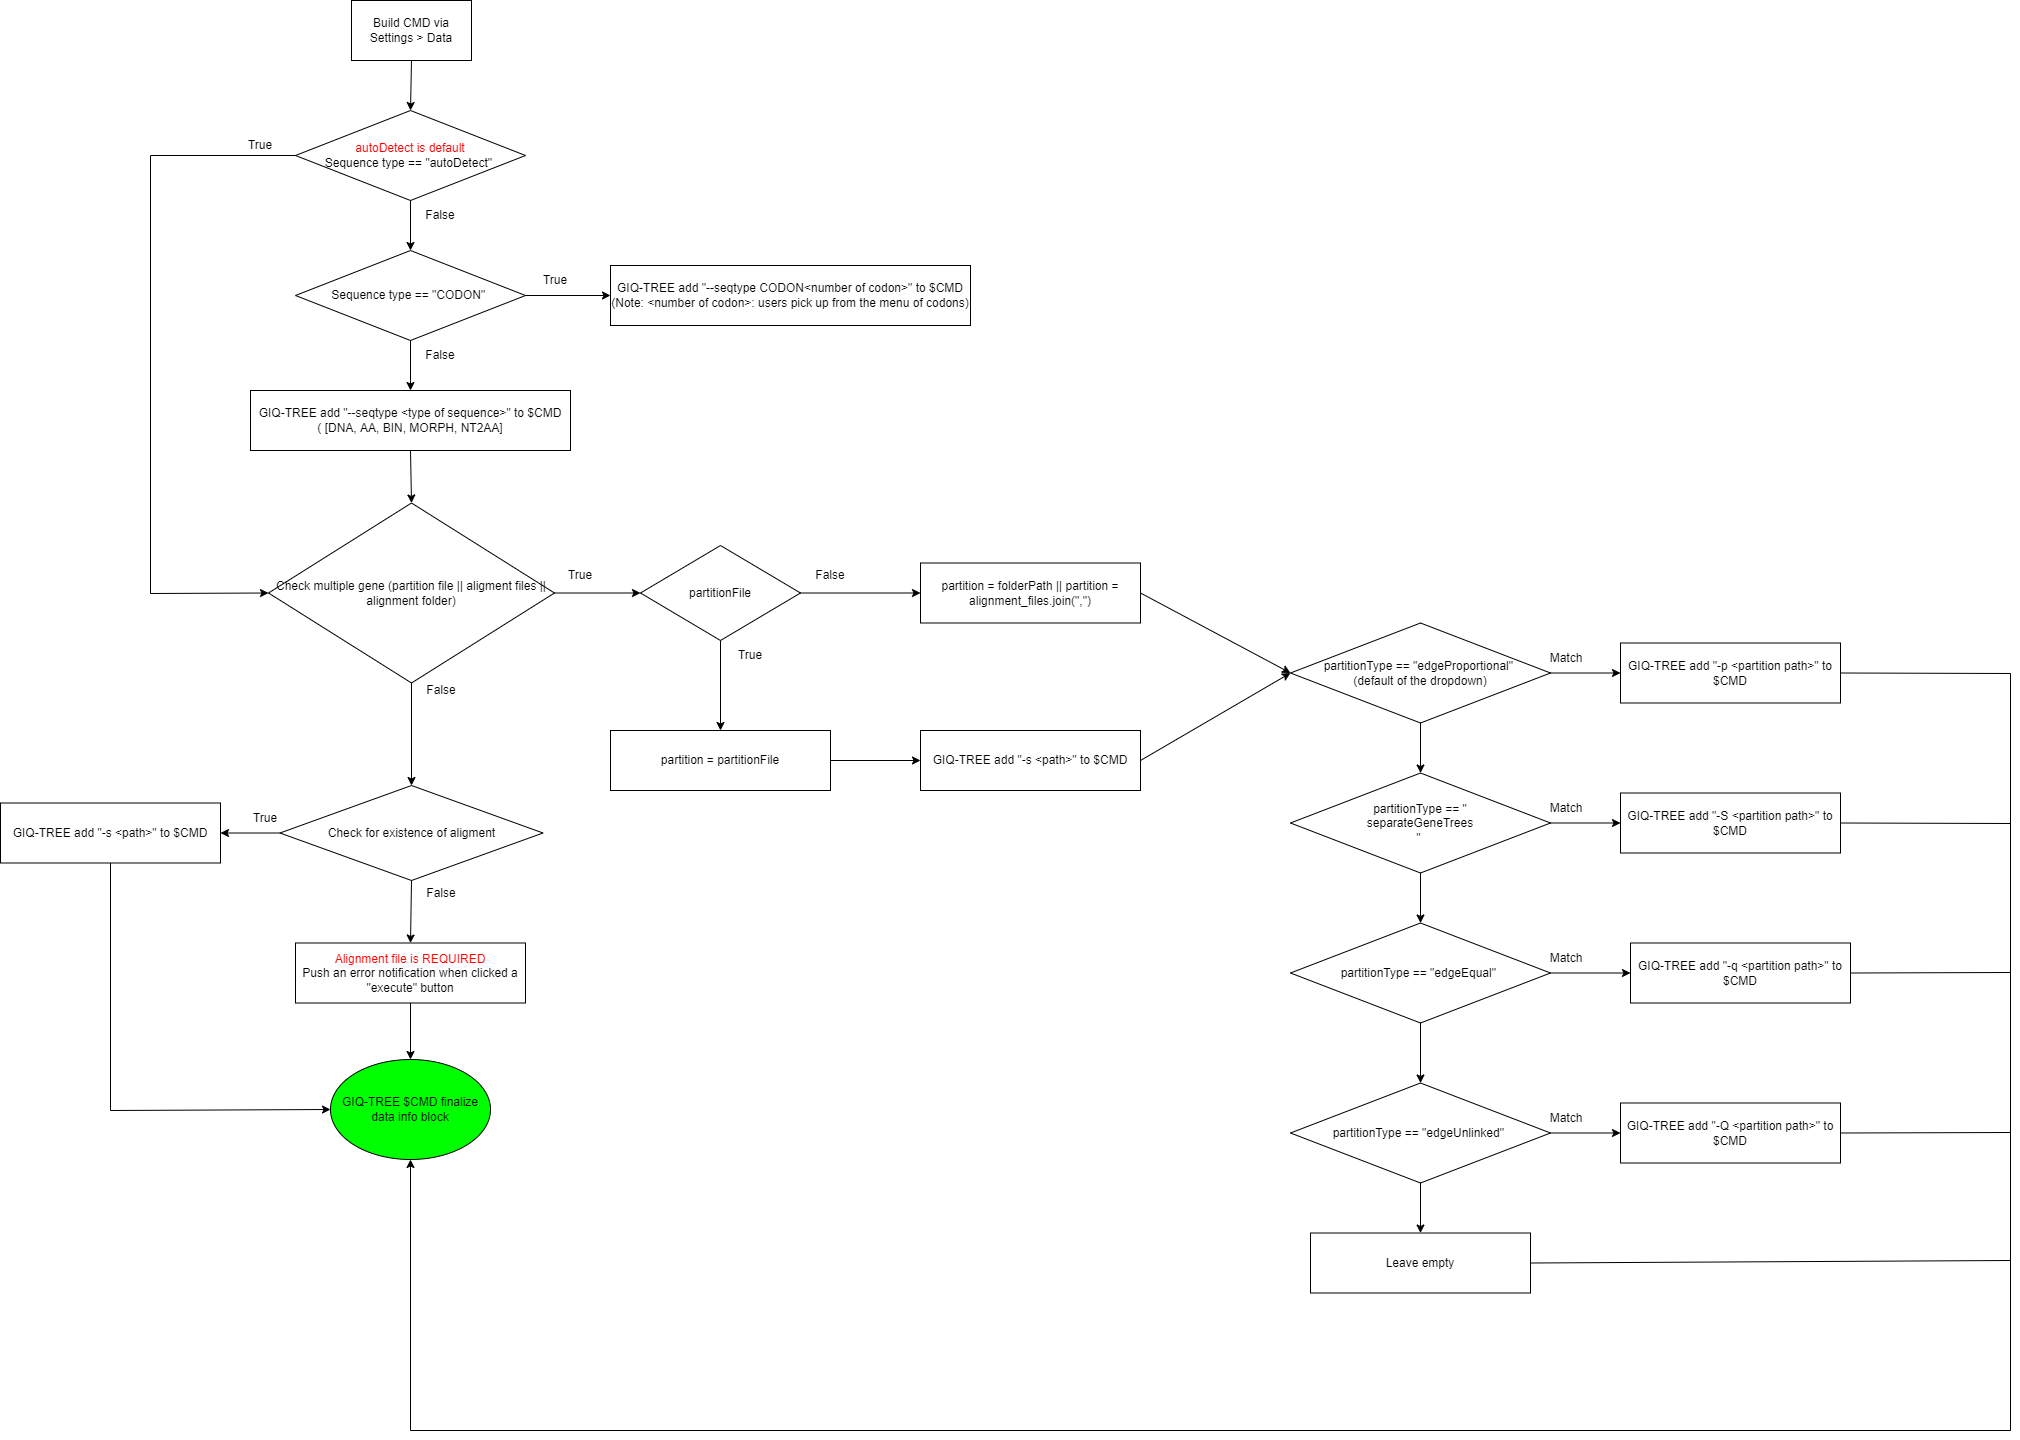
\includegraphics[scale=0.23]{Image/4.8.png}
	\caption{Luồng dữ liệu của phần dữ liệu trong cài đặt }
	\label{fig:image4.8}
\end{figure}

\subsection{Mô hình}
Nhánh mô hình là để tìm kiếm được cây phù hợp nhất với dữ liệu và yêu cầu bài toán đưa ra. Ở bước này, chúng ta cần lưu ý đến các trường dữ liệu như:

- Dữ liệu là đơn gene hay đa gene (được kiểm tra ở phần Data dựa vào alignment và partition)

- Các ràng buộc của kiểu dữ liệu tuần tự với từng mô hình

- Chỉ định mô hình biến đổi

- Chỉ định mô hình tần suất trạng thái (state frequency)

- Tùy chọn tự động ghép phân hoạch

- Thuật toán tự động ghép phân hoạch 

Các ràng buộc logic về các biến trong phần mô hình và luồng dữ liệu ánh xạ từ GIQ-TREE sang dòng lệnh IQTREE đã được mô tả chi tiết ở \textbf{Hình \ref{fig:image4.9}}

\begin{figure}[h]
	\centering
	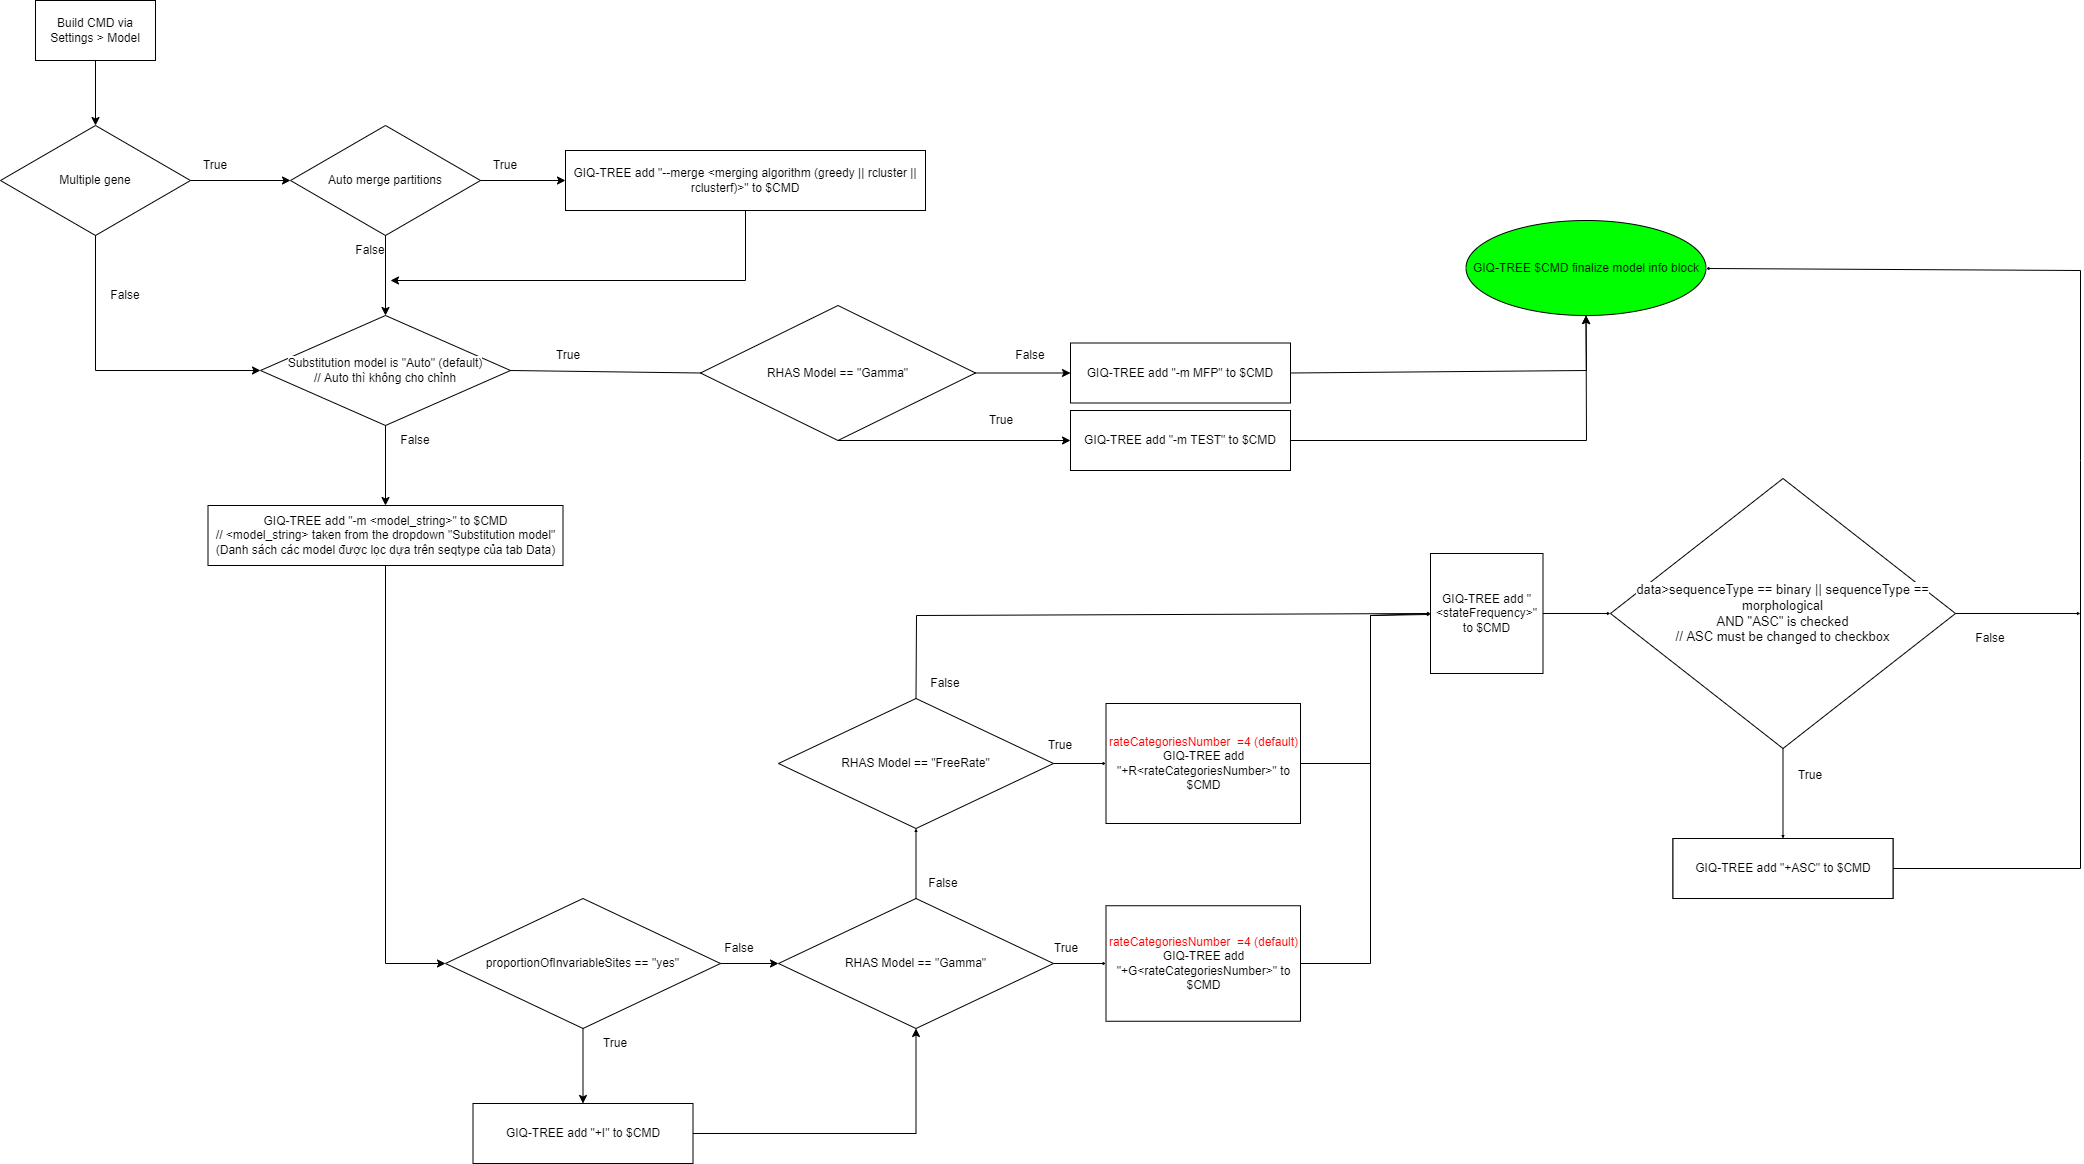
\includegraphics[scale=0.23]{Image/4.9.png}
	\caption{Luồng dữ liệu của cây tìm kiếm trong cài đặt }
	\label{fig:image4.9}
\end{figure}

\subsection{Tìm kiếm cây}
Tại mục này chúng ta cần quan tâm đến các trường dữ liệu như:

- Cây tìm kiếm có bật hay không?

- Điều kiện dừng khi tìm kiếm cây

- Mức độ phá cây khi làm tìm kiếm

- Cây khung được chỉ định khi nạp tệp đầu vào

- Cây tham chiếu được chỉ định khi nạp tệp đầu vào

Chi tiết được mô tả trong  \textbf{Hình \ref{fig:image4.10}}

\begin{figure}[h]
	\centering
	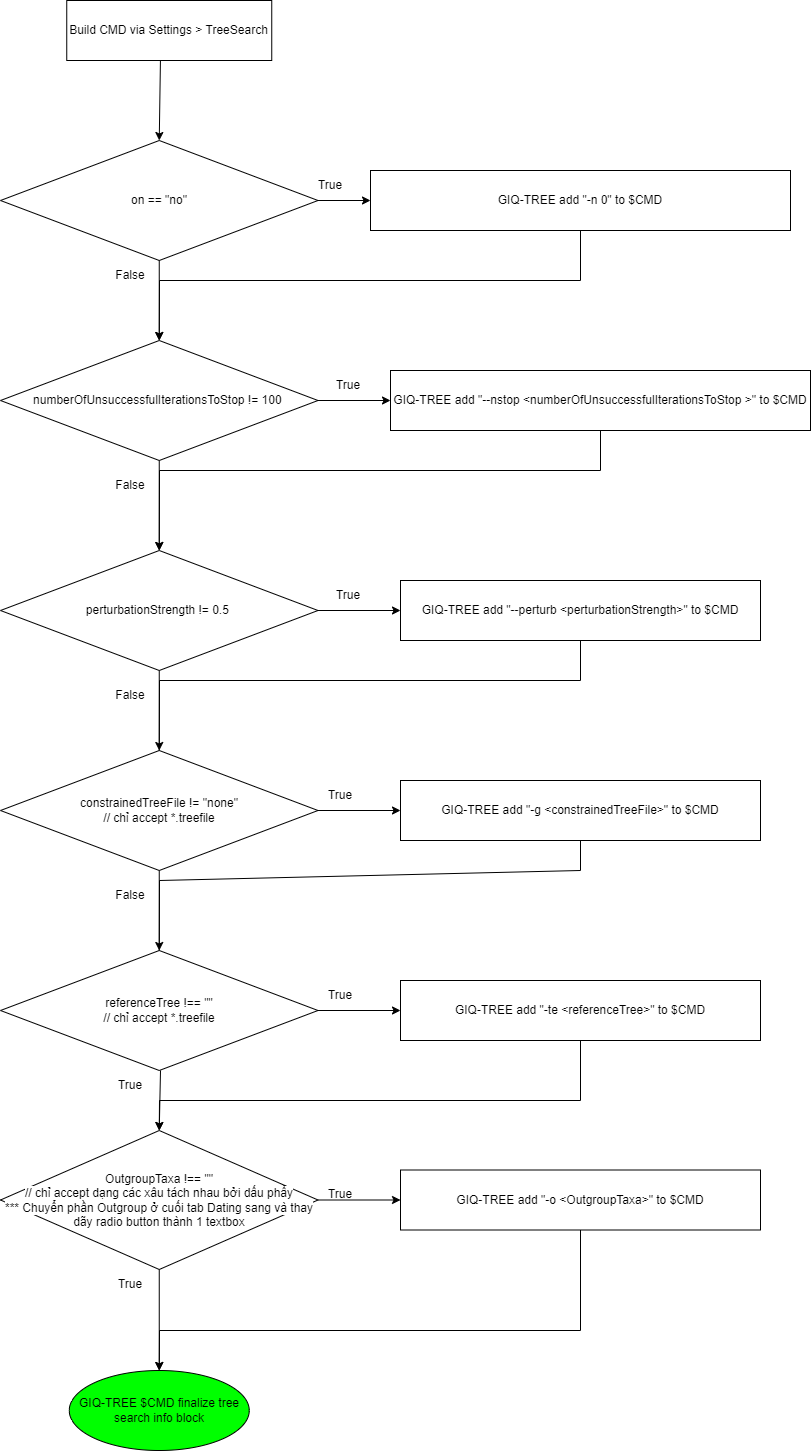
\includegraphics[scale=0.4]{Image/4.10.png}
	\caption{Luồng dữ liệu của phần cây tìm kiếm trong cài đặt }
	\label{fig:image4.10}
\end{figure}

\subsection{Hỗ trợ phân tích bootstrap}
Tại phần này, ứng dụng GIQ-TREE sẽ kiểm tra phương thức của cây bootstrap, tùy chọn UFBoot để giảm tác động của việc vi phạm nghiêm trọng mô hình, chiến lược lấy mẫu của các phân vùng, hay các kiểm tra trên cây đơn cũng như các yếu tố phù hợp (dạng tệp). Các trường dữ liệu cần lưu ý là:

- Phương pháp bootstrap sử dụng

- Tùy chọn bật thuật toán giảm vi phạm giả thiết mô hình kết hợp UFBoot

- Chỉ định phương pháp sinh sắp hàng bootstrap cho dữ liệu đa gen

- Tùy chọn kiểm định đơn cạnh

- Chỉ số tương thích giữa cây gen và cây loài

Chi tiết được mô tả ở  \textbf{Hình \ref{fig:image4.11}}

\begin{figure}[h]
	\centering
	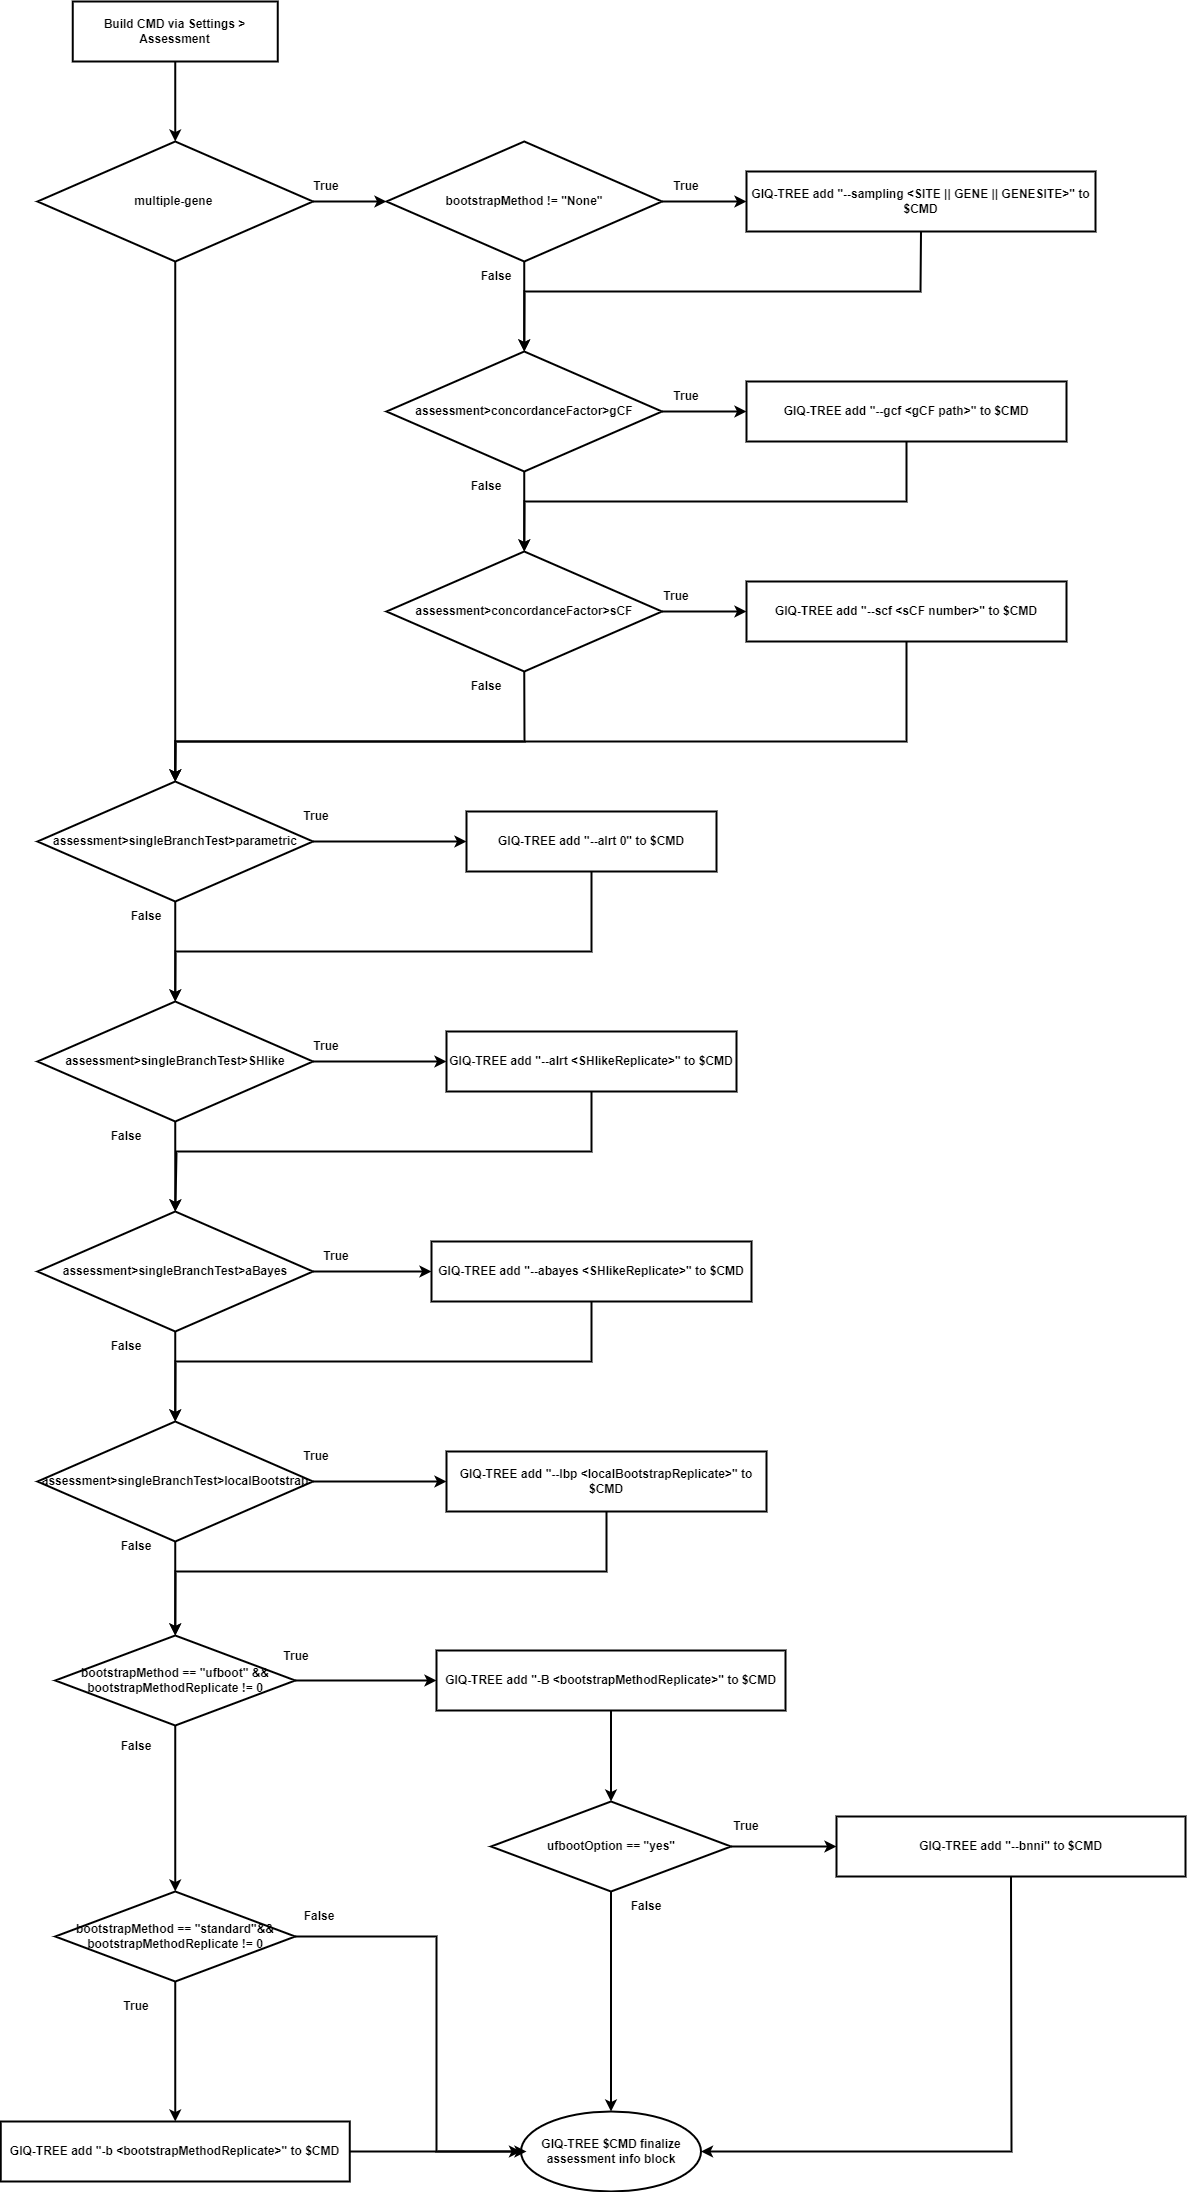
\includegraphics[scale=0.28]{Image/4.11.png}
	\caption{Luồng dữ liệu của hỗ trợ phân tích bootstrap trong cài đặt }
	\label{fig:image4.11}
\end{figure}

\subsection{Suy luận thời gian}
Tại phần này, ứng dụng sẽ kiểm tra xem có tồn tại thông tin về loại thời gian hay không? Từ đó đưa ra các câu lệnh phù hợp với dữ liệu. Các dữ liệu cần quan tâm là:

- Loại thông tin thời gian (lá/đỉnh trong)

- Chỉ định lấy thông tin thời gian từ tệp sắp hàng

- Tệp thời gian được chỉ định bằng tệp dữ liệu nạp vào

- Chỉ định cạnh gốc

 Chi tiết được mô tả thông qua  \textbf{Hình \ref{fig:image4.12}}

\begin{figure}[h]
	\centering
	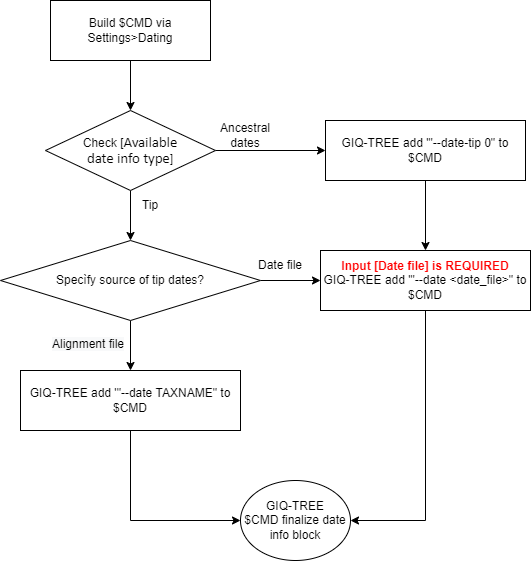
\includegraphics[scale=0.8]{Image/4.12.png}
	\caption{Luồng dữ liệu của thời gian trong cài đặt - hỗ trợ bời người hướng dẫn khoa học }
	\label{fig:image4.12}
\end{figure}

\subsection{Các tùy chọn cài đặt khác}
Ở phần cuối cùng này, các tùy chọn liên quan đến việc thêm các tinh chỉnh cài đặt khác người dùng muốn sử dụng (phần này sẽ được ghi đè khi thực hiện phân tích) hay lựa chọn đường dẫn lưu các tệp đầu ra và thay đổi các tùy chọn cài đặt mà tạo nên một cài đặt khác. Các trường dữ liệu cần quan tâm là:

- Chỉ định số luồng của sử dụng CPU 

- Mở rộng tham số

 Chi tiết được mô tả tại \textbf{Hình \ref{fig:image4.13}}
 
 \begin{figure}[h]
	\centering
	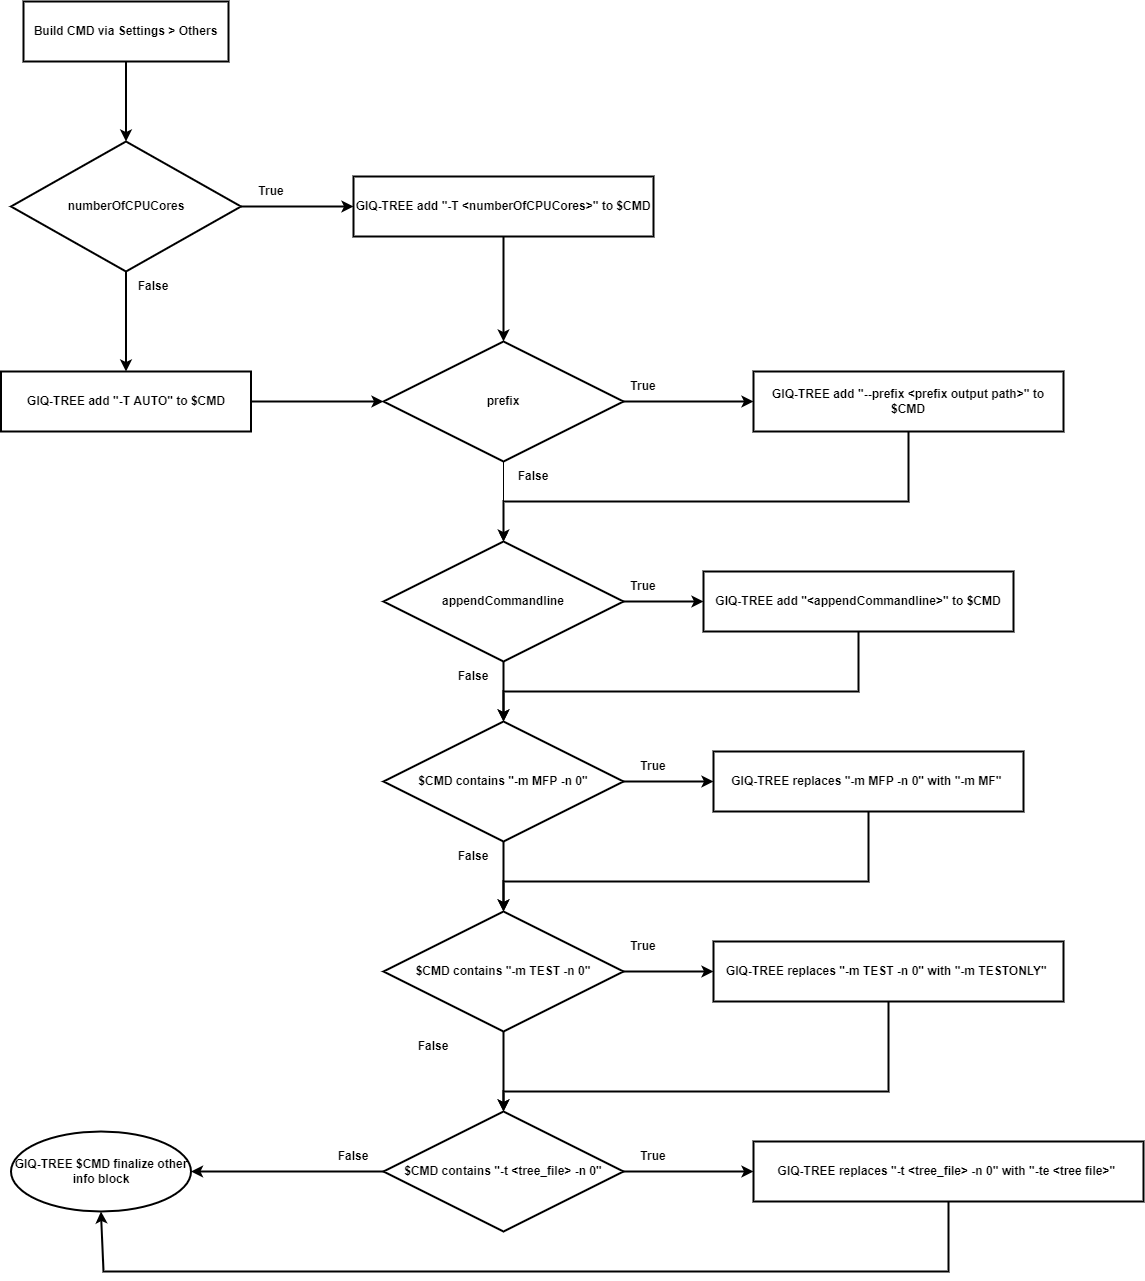
\includegraphics[scale=0.2]{Image/4.13.png}
	\caption{Luồng dữ liệu của tùy chọn cài đặt khác trong cài đặt }
	\label{fig:image4.13}
\end{figure}

\newpage	
\chapter{Hệ thống thực nghiệm}
\label{chap:chapter5}
\section{Chương trình thực nghiệm }
Chương trình được cài đặt và công khai mã nguồn tại \url{ https://github.com/sonntuet1997/gIqtree }

Ứng dụng phía back-end được thiết kế dưới dạng các sự kiện trả về dữ liệu để thuận tiện cho bên front-end xử lý về mặt hiển thị cũng như tách biệt được việc phát triển logic chính của ứng dụng và logic hiển thị cũng như hiển thị của ứng dụng. 
Ứng dụng back-end hoàn thiện được các chức năng như:

- Khởi tạo dự án

- Mở dự án đã tồn tại

- Xem các dự án đã được khởi tạo trước đó

- Tìm kiếm các dự án đã được khởi tạo trước đó

- Thực hiện tinh chỉnh dữ liệu trong cài đặt

- Thực hiện tinh chỉnh cài đặt mô hình

- Thực hiện tinh chỉnh cài đặt cây

- Thực hiện tinh chỉnh cài đặt hỗ trợ phân tích

- Thực hiện tinh chỉnh cài đặt hỗ trợ suy luận thời gian

- Thực hiện các tinh chỉnh cài đặt khác

Tệp chứa các dữ liệu tinh chỉnh cài đặt sẽ gồm các tham số và được bố trí như sau:

\begin{lstlisting}[language=Java,
caption={Dữ liệu cài đặt mặc định phân cấp với dự án kiểu Find Model },label={code:jdt-ast-gen}]
{
  projectType: "findmodel",
  status: "Empty",
  data: {
    alignment: "",
    partition: "",
    sequence: "autoDetect",
    codon: "codon1",
    partitionType: "separateGeneTrees",
  },
  model: {
    modelFinder: "auto",
    proportionOfInvariableSites: "no",
    rateCategories: "",
    rateCategoriesNumber: "4",
    autoMerge: "no",
    mergingAlgorithm: "",
    stateFrequency: "none",
  },
  tree: {
    on: "no",
    numberOfUnsuccessfulIterationsToStop: "100",
    perturbationStrength: "0.5",
    constrainedTreeFile: "",
    referenceTree: "",
  },
  assessment: {
    bootstrapMethod: "none",
    bootstrapMethodReplicate: "1000",
    ufbootOption: "no",
    multiPartitionSamplingStrategy: "SITE",
    singleBranchTest: {
      parametric: false,
      SHlike: false,
      aBayes: false,
      localBootstrap: false,
      SHlikeReplicate: "0",
      localBootstrapReplicate: "0",
    },
    concordanceFactor: {
      gCF: "",
      sCF: "",
    },
  },
  dating: {
    availableDateInfoType: "none",
    dateExtraction: "no",
    dateFile: "",
    branchContainingOutgroup: "autoDetect",
  },
  others: {
    numberOfCPUCores: "",
    prefix: "",
    enterCommandLine: "",
  },
}
\end{lstlisting}

\begin{lstlisting}[language=Java,
caption={Dữ liệu cài đặt mặc định phân cấp với dự án kiểu Merge Partitons },label={code:jdt-ast-gen}]
{
  projectType: "mergepartition",
  status: "Empty",
  data: {
    alignment: "",
    partition: "",
    sequence: "autoDetect",
    codon: "codon1",
    partitionType: "edgeProportional",
  },
  model: {
    modelFinder: "auto",
    proportionOfInvariableSites: "no",
    rateCategories: "",
    rateCategoriesNumber: "4",
    autoMerge: "yes",
    mergingAlgorithm: "rclusterf",
    stateFrequency: "none",
  },
  tree: {
    on: "no",
    numberOfUnsuccessfulIterationsToStop: "100",
    perturbationStrength: "0.5",
    constrainedTreeFile: "",
    referenceTree: "",
  },
  assessment: {
    bootstrapMethod: "none",
    bootstrapMethodReplicate: "1000",
    ufbootOption: "no",
    multiPartitionSamplingStrategy: "SITE",
    singleBranchTest: {
      parametric: false,
      SHlike: false,
      aBayes: false,
      localBootstrap: false,
      SHlikeReplicate: "0",
      localBootstrapReplicate: "0",
    },
    concordanceFactor: {
      gCF: "",
      sCF: "",
    },
  },
  dating: {
    availableDateInfoType: "none",
    dateExtraction: "no",
    dateFile: "",
    branchContainingOutgroup: "autoDetect",
  },
  others: {
    numberOfCPUCores: "",
    prefix: "",
    enterCommandLine: "",
  },
}
\end{lstlisting}

\begin{lstlisting}[language=Java,
caption={Dữ liệu cài đặt mặc định phân cấp với dự án kiểu Infer Tree },label={code:jdt-ast-gen}]
 {
  projectType: "infertree",
  status: "Empty",
  data: {
    alignment: "",
    partition: "",
    sequence: "autoDetect",
    codon: "codon1",
    partitionType: "edgeProportional",
  },
  model: {
    modelFinder: "auto",
    proportionOfInvariableSites: "no",
    rateCategories: "",
    rateCategoriesNumber: "4",
    autoMerge: "yes",
    mergingAlgorithm: "rclusterf",
    stateFrequency: "none",
  },
  tree: {
    on: "yes",
    numberOfUnsuccessfulIterationsToStop: "100",
    perturbationStrength: "0.5",
    constrainedTreeFile: "",
    referenceTree: "",
  },
  assessment: {
    bootstrapMethod: "ufboot",
    bootstrapMethodReplicate: "1000",
    ufbootOption: "no",
    multiPartitionSamplingStrategy: "SITE",
    singleBranchTest: {
      parametric: false,
      SHlike: false,
      aBayes: false,
      localBootstrap: false,
      SHlikeReplicate: "0",
      localBootstrapReplicate: "0",
    },
    concordanceFactor: {
      gCF: "",
      sCF: "",
    },
  },
  dating: {
    availableDateInfoType: "none",
    dateExtraction: "no",
    dateFile: "",
    branchContainingOutgroup: "autoDetect",
  },
  others: {
    numberOfCPUCores: "",
    prefix: "",
    enterCommandLine: "",
  },
}
\end{lstlisting}

\begin{lstlisting}[language=Java,
caption={Dữ liệu cài đặt mặc định phân cấp với dự án kiểu Assess Support },label={code:jdt-ast-gen}]
 {
  projectType: "assessment",
  status: "Empty",
  data: {
    alignment: "",
    partition: "",
    sequence: "autoDetect",
    codon: "codon1",
    partitionType: "edgeProportional",
  },
  model: {
    modelFinder: "auto",
    proportionOfInvariableSites: "no",
    rateCategories: "",
    rateCategoriesNumber: "4",
    autoMerge: "yes",
    mergingAlgorithm: "rclusterf",
    stateFrequency: "none",
  },
  tree: {
    on: "no",
    numberOfUnsuccessfulIterationsToStop: "100",
    perturbationStrength: "0.5",
    constrainedTreeFile: "",
    referenceTree: "",
  },
  assessment: {
    bootstrapMethod: "standard",
    bootstrapMethodReplicate: "1000",
    ufbootOption: "no",
    multiPartitionSamplingStrategy: "SITE",
    singleBranchTest: {
      parametric: false,
      SHlike: false,
      aBayes: false,
      localBootstrap: false,
      SHlikeReplicate: "0",
      localBootstrapReplicate: "0",
    },
    concordanceFactor: {
      gCF: "",
      sCF: "",
    },
  },
  dating: {
    availableDateInfoType: "none",
    dateExtraction: "no",
    dateFile: "",
    branchContainingOutgroup: "autoDetect",
  },
  others: {
    numberOfCPUCores: "",
    prefix: "",
    enterCommandLine: "",
  },
}
\end{lstlisting}

\begin{lstlisting}[language=Java,
caption={Dữ liệu cài đặt mặc định phân cấp với dự án kiểu Date Tree },label={code:jdt-ast-gen}]
{
  projectType: "datetree",
  status: "Empty",
  data: {
    alignment: "",
    partition: "",
    sequence: "autoDetect",
    codon: "codon1",
    partitionType: "edgeProportional",
  },
  model: {
    modelFinder: "auto",
    proportionOfInvariableSites: "no",
    rateCategories: "",
    rateCategoriesNumber: "4",
    autoMerge: "yes",
    mergingAlgorithm: "rclusterf",
    stateFrequency: "none",
  },
  tree: {
    on: "no",
    numberOfUnsuccessfulIterationsToStop: "100",
    perturbationStrength: "0.5",
    constrainedTreeFile: "",
    referenceTree: "",
  },
  assessment: {
    bootstrapMethod: "none",
    bootstrapMethodReplicate: "1000",
    ufbootOption: "no",
    multiPartitionSamplingStrategy: "SITE",
    singleBranchTest: {
      parametric: false,
      SHlike: false,
      aBayes: false,
      localBootstrap: false,
      SHlikeReplicate: "0",
      localBootstrapReplicate: "0",
    },
    concordanceFactor: {
      gCF: "",
      sCF: "",
    },
  },
  dating: {
    availableDateInfoType: "tip",
    dateExtraction: "no",
    dateFile: "",
    branchContainingOutgroup: "autoDetect",
  },
  others: {
    numberOfCPUCores: "",
    prefix: "",
    enterCommandLine: "",
  },
}
\end{lstlisting}

\section{Đánh giá phần mềm}
Hiệu năng thực hiện phân tích của phần mềm được đảm bảo do nhúng phần lõi của IQTREE vào bên trong và các thao tác bên cạnh đó thì gần như không ảnh hưởng đến hiệu năng khi thực hiện các phân tích.

Thật vậy, khi thử với bộ dữ liệu với các chức năng trên hai phiên bản IQTREE và GIQ-TREE trên cùng một cấu hình máy tính i7-8750H, GTX 1050Ti,  16GB, 256 SSD với cùng một tập dữ liệu, hiệu năng phân tích gần như giống nhau. Chi tiết xem tại \url{https://bit.ly/3K7jZac}

\newpage	
\chapter{Thảo luận và kết luận}
\label{chap:chapter6}

\section{Các nội dung nghiên cứu và phát triển được}
Trong khóa luận này, em đã tìm hiểu và xây dựng được phần back-end cho ứng dụng GIQ-TREE, một ứng dụng giao diện đồ họa người dùng đa nền tảng. Ngoài việc vận dụng được những kiến thức với kinh nghiệm trong việc phát triển phần mềm trước đó, em cũng học thêm được rất nhiều về quy trình nghiệp vụ cũng như việc giao tiếp, làm việc nhóm trong phát triển phần mềm. Chưa dừng ở đó, em còn tìm hiểu thêm được những kiến thức cơ bản trong lĩnh vực sinh học, tin sinh học. Quan trọng hơn cả, việc phát triển ứng dụng này khiến em thấy mình có ích khi góp một chút sức nhỏ để hỗ trợ và tiết kiệm thời gian hơn cho các nhà nghiên cứu nói chung và sinh học tiến hóa nói riêng. Em cũng học được một công nghệ mới là Electron.js để phát triển phần mềm ứng dụng máy tính (mảng em chưa từng thử sức trước đây). Em cũng học hỏi được rất nhiều từ góc nhìn cũng như kiến thức của những người đi trước và em vô cùng cảm kích về việc này

\newpage
\section{Nhận xét và hướng phát triển}
GIQ-TREE là một ứng dụng hay nhưng chưa đủ. Hiện nay, việc làm mịn ứng dụng vẫn còn đang được thực hiện do rất nhiều yếu tố khách quan cũng như chủ quan. Trong quá trình phát triển không tránh khỏi việc xuất hiện các lỗi và việc khắc phục là cần thiết để sản phẩm ổn định hơn. GIQ-TREE hướng đến một ứng dụng với độ ổn định cao và rất nhiều phiên bản trong tương lai sẽ được ra lò, chứ không dừng ở phiên bản chạy lần đầu (first-run) chỉ phục vụ cho việc học tập.

Trong tương lai, GIQ-TREE hướng đến việc thông minh hóa cũng như tối ưu thêm về trải nghiệm người dùng. GIQ-TREE trong các phiên bản tới sẽ thực hiện phân tích được với các tệp dữ liệu lớn và đem lại hiệu năng vượt trội hơn hiện nay.

Việc phát triển không chỉ do cá nhân em mà nó còn là công sức của cả tập thể hợp lại. Em rất vui khi là một cá thể nhỏ bé được góp sức trong một ứng dụng như GIQ-TREE.

\begin{thebibliography}{10}
\section*{Tiếng Việt}
	\bibitem{cia-0}
	Hoàng Thị Điệp. Các phương pháp nhanh xây dựng cây Bootstrap tiến hóa. \textit{Luận án tiến sĩ Công nghệ thông tin, Đại học Công nghệ - ĐHQGHN}, 2019.
	
\section*{Tiếng Anh}
    \bibitem{cia-1} 
	J. Felsenstein, Inferring phylogenies, 2nd ed. Sunderland (MA): Sinauer Associates, Inc, 2004.
	
	\bibitem{cia-2}
	Philippe Lemey, Marco Salemi, Anne-Mieke Vandamme, The Phylogenetic Handbook A Practical Approach to Phylogenetic Analysis and Hypothesis Testing , 2009

	\bibitem{cia-3} 
	L.-T. Nguyen, H. A. Schmidt, A. von Haeseler, and B. Q. Minh.
	“IQ-TREE: a fast and effective stochastic algorithm for estimating maximum-likelihood phylogenies,” \textit{Mol. Biol. Evol., vol. 32, no. 1, pp. 268–274} (2015).
	
	\bibitem{cia-4} 
	J. Trifinopoulos, L. T. Nguyen, A. von Haeseler, and B. Q. Minh, “W-IQ-TREE: a fast online phylogenetic tool for maximum likelihood analysis,” Nucleic Acids Res., vol. 44, no. W1, pp. W232–W235, Jul. 2016, doi: 10.1093/NAR/GKW256.
	
	\bibitem{cia-5} 
	A. Stamatakis, “RAxML version 8: a tool for phylogenetic analysis and post-analysis of large phylogenies,” Bioinformatics, vol. 30, no. 9, pp. 1312–1313, May 2014, doi: 10.1093/BIOINFORMATICS/BTU033.
	
	\bibitem{cia-6}
	D. Silvestro and I. Michalak, “raxmlGUI: a graphical front-end for RAxML,” Org. Divers. Evol. 2011 124, vol. 12, no. 4, pp. 335–337, Sep. 2011, doi: 10.1007/S13127-011-0056-0.
	
	\bibitem{cia-7}
	D. Edler, J. Klein, A. Antonelli, and D. Silvestro, “raxmlGUI 2.0: A graphical interface and toolkit for phylogenetic analyses using RAxML,” Methods Ecol. Evol., vol. 12, no. 2, pp. 373–377, Feb. 2021, doi: 10.1111/2041-210X.13512.
	
	\bibitem{cia-8}
	S. Guindon, J.-F. Dufayard, V. Lefort, M. Anisimova, W. Hordijk, and O. Gascuel, “New algorithms and methods to estimate maximum-likelihood phylogenies: assessing the performance of PhyML 3.0,” Syst. Biol., vol. 59, no. 3, pp. 307–321, 2010, doi: 10.1093/sysbio/syq010.
	
	\bibitem{cia-9}
	PHYML Online—a web server for fast maximum likelihood-based phylogenetic inference
	
	\bibitem{cia-10}
	J. C. Masters and L. Pozzi, “Phylogenetic Inference,” Int. Encycl. Primatol., pp. 1–6, Apr. 2017, doi: 10.1002/9781119179313.WBPRIM0419.
	
	\bibitem{cia-11}
	N. Saitou and M. Nei, “The neighbor-joining method: a new method for reconstructing phylogenetic trees,” Mol. Biol. Evol., vol. 4, no. 4, pp. 406–425, 1987.
	
	\bibitem{cia-12}
	W. M. Fitch, “Toward defining the course of evolution: minimum change for a specific tree topology,” Syst. Zool., vol. 20, no. 4, pp. 406–416, 1971.
	
	\bibitem{cia-13} 
	S. Guindon, J.-F. Dufayard, V. Lefort, M. Anisimova, W. Hordijk, and O. Gascuel, “New algorithms and methods to estimate maximum-likelihood phylogenies: assessing the performance of PhyML 3.0,” Syst. Biol., vol. 59, no. 3, pp. 307–321, 2010, doi: 10.1093/sysbio/syq010.
	
	\bibitem{cia-14}
	H. A. Schmidt, K. Strimmer, M. Vingron, and A. von Haeseler, “TREE-PUZZLE: maximum likelihood phylogenetic analysis using quartets and parallel computing,” Bioinformatics, vol. 18, no. 3, pp. 502–504, 2002, doi: 10.1093/bioinformatics/18.3.502.
	
    \bibitem{cia-15}
	B. Q. Minh et al., “IQ-TREE 2: New Models and Efficient Methods for Phylogenetic Inference in the Genomic Era,” Mol. Biol. Evol., vol. 37, no. 5, pp. 1530–1534, 2020.
\end{thebibliography}

\end{document}
